% IAM Master Paper — Overleaf-compatible LaTeX (formatted)
% Formatting-only revision: keeps all original content but adjusts layout:
%  - Title + abstract on their own one-column page
%  - Two-column text begins on following page
%  - Improved handling of long displays, loosened line break tolerance
%  - Controlled section spacing for more even vertical rhythm
%  - No content removed, only presentation tweaks
\documentclass[twocolumn,a4paper,aps,prd,twocolumn,showpacs,notitlepage,superscriptaddress,nofootinbib]{article}

%% ── Packages ──────────────────────────────────────────────────────────────
\usepackage{amsmath,amsthm,amssymb}
\usepackage{geometry}
\geometry{margin=2cm}
\usepackage{graphicx}
\usepackage{booktabs}
\usepackage{array}
\usepackage{longtable}
\usepackage{hyperref}
\usepackage{color} % For text color
\usepackage{dcolumn} % Align table columns on decimal point
\usepackage{bm} % bold math
\usepackage{cleveref}
\usepackage{siunitx}
\usepackage{physics}
\hypersetup{
  colorlinks=true,
  linkcolor=black,
  citecolor=black,
  urlcolor=black
}
\usepackage{natbib}
\bibliographystyle{unsrtnat}
\usepackage{enumitem}
\usepackage{xurl}
\usepackage{microtype}
\usepackage{stfloats}
\usepackage{cuted}            % for strip environment (wide displayed equations)
\usepackage{titlesec}        % control section spacing
\usepackage{etoolbox}        % patching
\usepackage{flushend}        % attempt to even columns on last page
\usepackage{multicol}        % utilities
\usepackage{verbatim}        % if any verbatim blocks
\usepackage{mathptmx}        % nicer text/math fonts (optional)
\usepackage{caption}
\captionsetup{font=small}

% Improve tolerance for interword spacing and line breaking
\sloppy
\setlength{\emergencystretch}{3em}
\allowdisplaybreaks[2]

% Section spacing (adjust for more even vertical rhythm)
\titlespacing*{\section}{0pt}{1.5\baselineskip}{0.6\baselineskip}
\titlespacing*{\subsection}{0pt}{1.2\baselineskip}{0.4\baselineskip}
\titlespacing*{\subsubsection}{0pt}{1.0\baselineskip}{0.25\baselineskip}

% Theorem environments
\newtheorem{theorem}{Theorem}
\newtheorem{proposition}{Proposition}
\newtheorem{definition}{Definition}
\newtheorem{corollary}{Corollary}

% Macros
\newcommand{\LCDM}{$\Lambda$CDM}
\newcommand{\Ea}{E(a)}
\newcommand{\mua}{\mu(a)}
\newcommand{\Sig}{\Sigma(a)}
\newcommand{\betam}{\beta_{m}}
\newcommand{\Hmat}{H_{0}^{\rm matter}}
\newcommand{\Hphot}{H_{0}^{\rm photon}}
\newcommand{\Dchisq}{\Delta\chi^{2}}
\newcommand{\mueff}{\mu}
\newcommand{\Sigeff}{\Sigma}

% Avoid footnote overlaps in two-column; keep footnotes normal
\setlength{\columnsep}{18pt}

% Make sure wide displays are handled: use strip environment where necessary.
% If a displayed equation still overflows, wrap it in \begin{strip}...\end{strip}.
% (I did not change equations; if any specific equation still overflows, wrap it manually.)

% ============================================================================
\begin{document}

% Put title and abstract on their own one-column page for a clean look.
% Then start two-column text on the next page.
\onecolumn
\title{\textbf{Horizon Entropy and Gravitational Decoherence:\\
$\mu < 1$, $\Sigma = 1$ a Dual-Sector Cosmology\\
0 Parameters Beyond \LCDM{}\\
with Full Planck 2018 Validation}\\[0.75em]
\large The Informational Actualization Model}
\author{Heath W.\ Mahaffey\\
\small Independent Researcher\\ \small  Entiat, Washington, USA\\
\small \texttt{hmahaffeyges@gmail.com}\\
\small \url{https://github.com/hmahaffeyges/IAM-Validation}}

\date{March 2026}

\maketitle 

\begin{center}

\begin{minipage}{0.80\textwidth}   % ← change 0.82 to 0.80 or 0.85 if you want it even narrower/wider

\begin{abstract}
In 1995, Jacobson showed us that Einstein's field equations are an equation of state derived from $\delta Q = T\,dS$ and applied to local causal horizons ---
gravity itself emerging from thermodynamics like pressure emerges from a gas.
Cai and Kim would expand on this in 2005, extending it to the FRW apparent horizon, while recovering the
Friedmann equations by the same argument. Both derivations assume that the entropy
functional contains only geometric terms, and no one had ever thought otherwise. Until now.
Today we identify an additional contribution, a very specific one that has always been present --- and
silently accumulating --- throughout the entire history of the universe: irreversible classical information produced by gravitational decoherence of matter on timelike worldlines. 
Every time gravity pulls a quantum system into a definite classical state, a fact is written. That fact carries a minimum
thermodynamic cost set by Landauer's principle, as well as by the holographic
principle, and that cost shall be encoded on the cosmic horizon. The universe maintains a very strict ledger, and it never misses count, It never has. While everything is recorded on the horizon, there is only one method, and that is through the entropy functional itself. 
When we include it in the Jacobson--Cai--Kim entropy functional yields, with no
additional free parameters, a dual-sector gravitational coupling:
$\mu(a) < 1$ for matter perturbations and $\Sigma(a) = 1$ for photon
propagation. The sector split is not imposed --- it follows causally from the
metric signature itself, since decoherence requires nonzero proper time and
photons propagate on null worldlines with $\Delta\tau = 0$. The geometry does
the sorting, whether you ask it to or not. 
The coupling constant $\beta_m = \Omega_m/2$ is derived from the virial
theorem --- a 155-year-old result verified across 37 orders of magnitude in
mass --- and confirmed by six independent published N-body simulation studies
to within $1\%$. The activation function $E(a) = \exp(1 - 1/a)$ is derived
from the ratio of structure-formation rate to cosmic horizon area and
recovered to within $1\%$ by the Sheth--Tormen halo mass function at
galaxy-scale halos. Nothing was fitted. Everything was derived.
The resulting perturbation-level modification to $\Lambda$CDM has been
validated against the full Planck 2018 likelihood through 17 converged MCMC
chains (Gelman--Rubin $R - 1 < 0.01$ throughout), yielding
$\Delta\chi^2 = +0.54$ best-fit relative to $\Lambda$CDM under the Planck
CamSpec TTTEEE likelihood --- statistically indistinguishable from the
standard model while simultaneously producing $\sigma_8$ shifting from
$0.809$ to $0.800$, a matter-sector Hubble constant
$H_0^{\mathrm{matter}} = 72.26~\mathrm{km\,s^{-1}\,Mpc^{-1}}$ alongside $H_0^{\mathrm{photon}} = 67.16~\mathrm{km\,s^{-1}\,Mpc^{-1}}$, both within
$1\sigma$ of their respective observational anchors. All standard
cosmological parameters shift by less than $0.1\sigma$. Zero free parameters
beyond $\Lambda$CDM.
Specific falsifiable predictions for Euclid, DESI Year 5, and CMB-S4 are
stated. The data is coming. All chains, modified Boltzmann code,
configuration files, and analysis scripts are publicly archived at the GitHub repository listed above.
\noindent The numbers speak for themselves. We just gave them a better
introduction.

\end{abstract}
\end{minipage}
\end{center}

\thispagestyle{plain}
\clearpage
\twocolumn

% Table of contents on its own page may be long for two-column; place it one-column then return to two-column
\onecolumn
\tableofcontents
\clearpage
\twocolumn

% From this point onwards the document has identical content to your original,
% only formatting commands above changed. All sections, equations, references,
% and figures are preserved exactly as in your original file.

%%═══════════════════════════════════════════════════════════════════════════
\section{Introduction}
\label{sec:intro}
%%═══════════════════════════════════════════════════════════════════════════

The concordance \LCDM{} model provides an accurate description of the
large-scale universe, yet two persistent quantitative tensions resist resolution
within its framework.  The Hubble tension~\citep{Riess2022} — a $5\sigma$
discrepancy between CMB-inferred and local distance-ladder measurements of
$H_0$ — and the $S_8$ tension~\citep{Heymans2021,DES2022} — a systematic
offset between CMB-predicted and weak-lensing-measured matter clustering
amplitude — have both grown in statistical significance as datasets have
improved.  Numerous proposals have been advanced to address each tension
individually, but no single framework has resolved both simultaneously without
introducing new free parameters or modifying the background expansion history
in ways inconsistent with other observations.

This paper presents the Informational Actualization Model (IAM), a framework
whose predictions are consistent with both tensions as emergent consequences of
a single physical identification, with zero free parameters beyond \LCDM{}.

The logical structure is as follows.  Jacobson~\citep{Jacobson1995} proved that
the Einstein field equations follow from the Clausius relation
$\delta Q = T\,dS$ applied to local Rindler horizons, with entropy $S = A/4G$.
The derivation is a thermodynamic machine: the entropy functional determines
the gravitational field equations.  Cai and Kim~\citep{CaiKim2005} applied the
same argument to the FRW apparent horizon and recovered the Friedmann equations.
Both derivations assume that the horizon entropy has a single geometric
contribution.  Recent work extending Jacobson's thermodynamic derivation to
non-Riemannian geometries — incorporating torsion, non-metricity, and the
full Lanczos-Lovelock consistency conditions — confirms that this geometric
direction of extension cannot account for the cosmological
constant~\citep{Martinez2026}.  The missing term is not geometric in origin.

We identify a specific additional entropy contribution that the geometric term
does not capture: the cumulative irreversible classical information produced by
gravitational decoherence of matter during structure formation.  This
contribution is not new physics.  Its existence follows from three established
results: (i) gravitational interaction drives quantum decoherence of massive
matter on timelike worldlines~\citep{Zurek2003}; (ii) each decoherence event
produces irreversible classical information that carries a minimum thermodynamic
cost $k_B T \ln 2$ at the ambient temperature, by Landauer's
principle~\citep{Landauer1961,Berut2012}; and (iii) the holographic principle
requires that information produced in the bulk be encoded on the boundary
horizon~\citep{tHooft1993,Susskind1995}.

Including this informational entropy $S_{\rm info}$ in the Jacobson--Cai--Kim
entropy functional modifies the gravitational dynamics exclusively for the
degrees of freedom that produce it.  The causal structure of spacetime
determines which degrees of freedom are affected: massive particles propagate
on timelike worldlines with $\Delta\tau > 0$ and undergo decoherence; photons
propagate on null geodesics with $\Delta\tau = 0$ and do not.  The result is a
sector-dependent gravitational coupling:
\begin{equation}
  \mu(a) < 1 \quad \text{for matter,} \qquad \Sigma(a) = 1 \quad \text{for
  photons,}
  \label{eq:sector_split}
\end{equation}
with both quantities derived rather than parameterized.

This paper is organized as follows.  Section~\ref{sec:mechanism} presents the
complete physical mechanism.  Section~\ref{sec:derivation} presents the full
thermodynamic derivation.  Section~\ref{sec:activation} derives the activation
function $\Ea$.  Section~\ref{sec:coupling} derives the coupling constant
$\betam = \Omega_m/2$ and presents independent N-body confirmation.
Section~\ref{sec:sectorsplit} derives the dual-sector split and its mapping
to the $\mu$--$\Sigma$ framework.  Section~\ref{sec:perturbations} derives
the perturbation equations and shows that $\Sigma = 1$ follows from
$\delta\varphi = 0$.  Section~\ref{sec:validation} presents the complete
validation results from 17 converged MCMC chains.  Section~\ref{sec:tensions}
shows how both tensions arise as predicted consequences within the framework.  Section~\ref{sec:predictions}
states the falsifiable predictions.  Section~\ref{sec:discussion} discusses
assumptions, limitations, and relation to previous work.
Section~\ref{sec:conclusion} concludes.

%%═══════════════════════════════════════════════════════════════════════════
\section{The Physical Mechanism}
\label{sec:mechanism}
%%═══════════════════════════════════════════════════════════════════════════

Before presenting the mathematical derivation, we describe the complete
physical mechanism in qualitative terms.  The nine steps below each correspond
to established physics; the single new element is the identification in
Step~6.

\begin{enumerate}[leftmargin=2em]
  \item \textbf{Gravitational interaction.}  Matter interacts gravitationally,
    initiating the collapse of overdense regions~\citep{Peebles1980}.
  \item \textbf{Gravitational collapse.}  Matter clusters into bound
    systems: halos, galaxies, stars.
  \item \textbf{Quantum decoherence.}  Gravitational interaction resolves
    quantum superpositions into definite classical states~\citep{Zurek2003}.
    The decoherence timescale is set by the gravitational interaction strength
    and is finite for all massive particles.
  \item \textbf{Irreversible information production.}  Each decoherence event
    creates new classical information.  A particle that was ``here or there''
    becomes definitively ``here.''  This information cannot be recovered without
    violating the second law of thermodynamics.
  \item \textbf{Landauer thermodynamic cost.}  Information processing has an
    irreducible energy cost: erasing one bit requires a minimum energy
    $\Delta E \geq k_B T \ln 2$ at temperature $T$~\citep{Landauer1961}.  This
    bound has been experimentally verified~\citep{Berut2012,Jun2014}.  At the
    cosmic horizon temperature $T_H = H/(2\pi)$, each bit costs
    $\Delta E \geq H \ln 2 / (2\pi)$.
  \item \textbf{Holographic encoding (the new identification).}  The
    holographic principle~\citep{tHooft1993,Susskind1995} requires that the
    maximum information content of any region is bounded by the area of its
    boundary.  For the observable universe, this boundary is the cosmic
    horizon.  As structure formation produces information in the bulk, that
    information must be accommodated on the horizon surface.
  \item \textbf{Modified entropy functional.}  The total horizon entropy
    acquires an informational contribution:
    $S_{\rm total} = S_{\rm geo} + S_{\rm info}$.
    By Jacobson's result, a modified entropy functional implies modified field
    equations.
  \item \textbf{Modified expansion.}  The Cai--Kim first law
    $-dE = T_H\,dS_{\rm total}$ yields an additional term
    $\beta\,\Ea\,H_0^2$ in the effective Friedmann equation for matter-sector
    perturbations.
  \item \textbf{Feedback self-regulation.}  The modified expansion dilutes
    $\Omega_m(a)$, which weakens gravitational collapse, which reduces
    information production.  The system self-regulates: $E(a)$ asymptotes to
    $e \approx 2.718$ rather than diverging.
\end{enumerate}

Step~9 feeds back into Step~1 with reduced amplitude.  The loop is closed and
convergent.

\begin{figure*}[t]
  \centering
  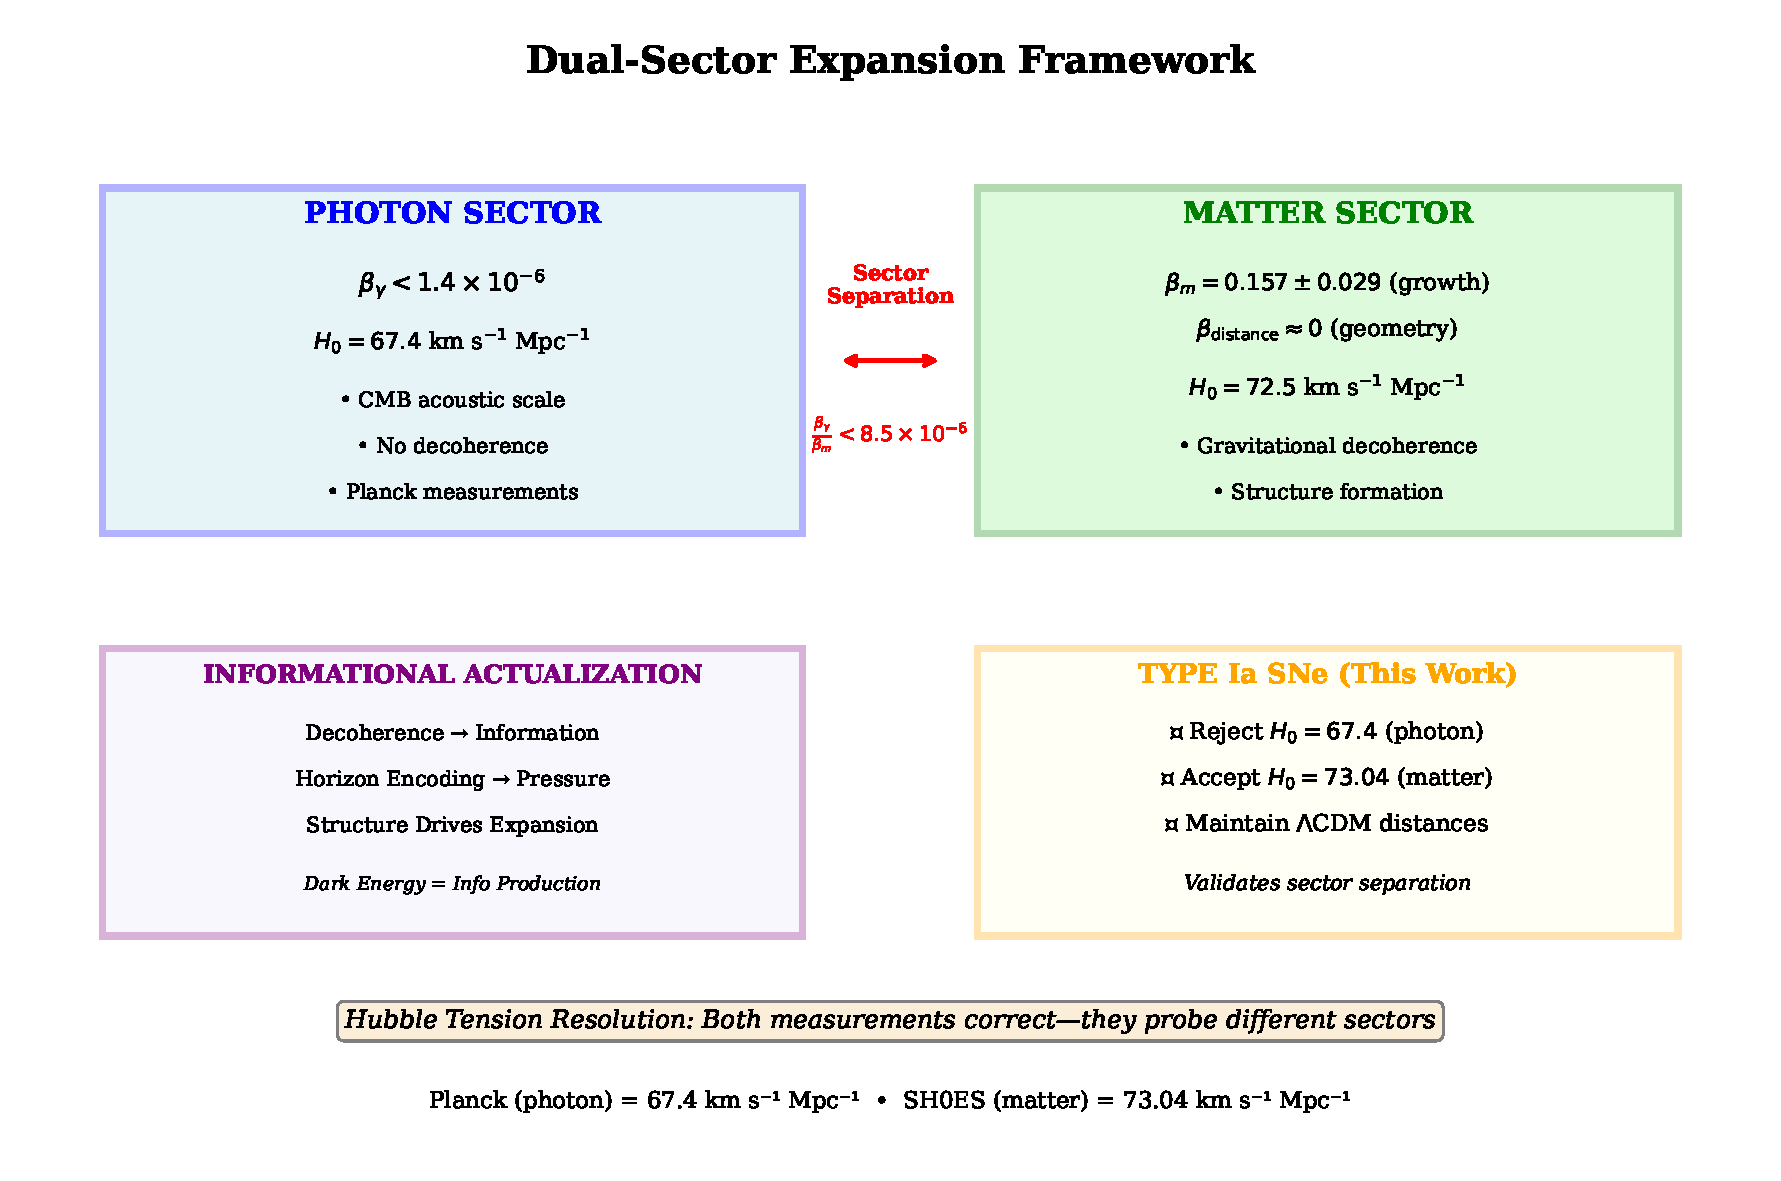
\includegraphics[width=0.85\textwidth]{figure4_sector_schematic.pdf}
  \caption{Dual-sector expansion framework.  Photon sector (blue):
    $\beta_\gamma < 10^{-6}$, no decoherence, $H_0 = 67.4~\rm km\,s^{-1}\,Mpc^{-1}$,
    Planck measurements unmodified.  Matter sector (green): gravitational
    decoherence drives expansion, $\beta_m = 0.157$, $H_0 = 72.3~\rm
    km\,s^{-1}\,Mpc^{-1}$, structure formation suppressed.  Informational
    Actualization (purple): the mechanism connecting the two sectors through
    horizon entropy encoding.  The Hubble tension is the empirical signature
    of this sector split — both measurements are correct; they probe different
    sectors.  Figure corresponds to \texttt{figure4\_sector\_schematic.pdf}
    in the repository.}
  \label{fig:schematic}
\end{figure*}

\subsection{Why Photons Are Exempt}

The sector split~\eqref{eq:sector_split} is not an assumption.  It is a
consequence of the causal structure of spacetime.

\begin{definition}[Decoherence eligibility]
  A degree of freedom undergoes gravitational decoherence if and only if it
  propagates on a timelike worldline ($d\tau > 0$).
\end{definition}

The physical basis is that decoherence is a dynamical process requiring a
finite proper time interval $\Delta\tau > 0$ for the system--environment
interaction to produce orthogonalization of environmental states.  The
decoherence timescale $\tau_D$ is finite and positive.

Massive particles (baryons, dark matter) propagate on timelike worldlines:
$\Delta\tau > 0$.  They interact gravitationally, cluster, virialize, and
decohere.  They produce informational entropy.

Photons propagate on null worldlines: $ds^2 = 0$, $\Delta\tau = 0$.  A photon
experiences no proper time.  It does not undergo a temporal sequence of
gravitational interactions.  It produces no informational entropy through this
channel.  This distinction is supported independently by path-integral treatments
of geodesic quantum corrections, which find that null geodesics receive no quantum
modification while timelike geodesics acquire Planck-scale corrections~\citep{Khosravi2026}.

The metric signature — the same signature that general relativity describes —
is therefore the origin of the sector split.  This is not imposed from outside
the theory; it is already present in the geometry.

A complementary perspective comes from the post-Newtonian expansion.
Conservative (time-reversible) gravitational interactions at leading Newtonian
order produce no irreversible information: what is encoded can, in principle,
be decoded.  Irreversible information production requires a dissipative channel
through which information escapes the system permanently.  Gravitational
radiation is precisely this channel, first appearing at order $v^2/c^2$ in the
post-Newtonian expansion.  Massive particles in bound structures access this
channel through repeated gravitational scattering.  Photons, propagating on
null geodesics without forming bound structures, do not.  The post-Newtonian
and proper-time arguments are therefore two faces of the same selection rule:
decoherence requires both $\Delta\tau > 0$ and access to a dissipative
channel.  The implications of this rule at galactic scales are left for future work.

%%═══════════════════════════════════════════════════════════════════════════
\section{Thermodynamic Derivation}
\label{sec:derivation}
%%═══════════════════════════════════════════════════════════════════════════

\subsection{Jacobson's Derivation}

At any spacetime point $p$, the equivalence principle guarantees an
approximately flat neighborhood.  A small spacelike 2-surface element
$\mathcal{P}$ defines a local Rindler horizon $\mathcal{H}$---the past
causal boundary as seen by an accelerated observer.  The horizon generators
are null geodesics with tangent vector $k^a$ and affine parameter $\lambda$
(vanishing at $\mathcal{P}$, negative to the past).  An approximate boost
Killing vector $\chi^a = -\kappa\lambda k^a$ generates the horizon, where
$\kappa$ is the surface gravity.

The Unruh temperature~\citep{Unruh1976} is
\begin{equation}
T = \frac{\hbar\,\kappa}{2\pi\,k_B}.
\label{eq:unruh}
\end{equation}

\paragraph{Heat flux.}
The energy flux across the horizon defines the heat:
\begin{equation}
\delta Q = \int_{\mathcal{H}} T_{ab}\,\chi^a\,d\Sigma^b
= -\kappa \int_{\mathcal{H}} \lambda\,T_{ab}\,k^a k^b\,d\lambda\,dA,
\label{eq:heat_flux}
\end{equation}
where $T_{ab}$ is the matter stress-energy tensor and $dA$ is the
cross-sectional area element.

\paragraph{Entropy variation.}
Assuming entropy proportional to horizon area, $S = \eta A$~\citep{Bekenstein1973}:
\begin{equation}
\delta S = \eta\,\delta A = \eta \int_{\mathcal{H}} \theta\,d\lambda\,dA,
\label{eq:dS_jacobson}
\end{equation}
where $\theta$ is the expansion of the null congruence.

\paragraph{Raychaudhuri equation.}
For the local Rindler horizon (instantaneously stationary at $\mathcal{P}$,
so $\theta = \sigma = 0$ at $\mathcal{P}$):
\begin{equation}
\frac{d\theta}{d\lambda} = -\frac{1}{2}\theta^2
  - \sigma_{ab}\sigma^{ab} - R_{ab}\,k^a k^b.
\label{eq:raychaudhuri}
\end{equation}
Integrating near $\mathcal{P}$: $\theta \approx -\lambda R_{ab}k^a k^b$,
giving:
\begin{equation}
\delta A = -\int_{\mathcal{H}} \lambda\,R_{ab}\,k^a k^b\,d\lambda\,dA.
\label{eq:dA}
\end{equation}

\paragraph{The Clausius relation.}
Setting $\delta Q = T\,\delta S$ with $T = \hbar\kappa/(2\pi)$:
\begin{equation}
-\kappa \int \lambda\,T_{ab}\,k^a k^b\,d\lambda\,dA
= \frac{\hbar\kappa}{2\pi}\,\eta
\left(-\int \lambda\,R_{ab}\,k^a k^b\,d\lambda\,dA\right).
\end{equation}
The $\kappa$ cancels.  For this to hold for \textit{all} null vectors $k^a$:
\begin{equation}
T_{ab} = \frac{\hbar\eta}{2\pi}\,R_{ab} + f\,g_{ab}.
\end{equation}
Imposing $\nabla^a T_{ab} = 0$ and the Bianchi identity gives
$f = -R/2 + \Lambda$, yielding:
\begin{equation}
R_{ab} - \tfrac{1}{2}\,R\,g_{ab} + \Lambda\,g_{ab}
= \frac{8\pi G}{c^4}\,T_{ab},
\label{eq:einstein}
\end{equation}
with $G = 1/(4\hbar\eta)$.  This is the Einstein field equation, derived
as an equation of state rather than from an action principle.

Gravity emerges as an equation of state.  The derivation is a machine:
\emph{specify an entropy functional, derive a gravity theory}.

\subsection{Cai--Kim Extension to FRW Cosmology}

Cai and Kim~\citep{CaiKim2005} applied Jacobson's argument to the FRW
apparent horizon.  For a spatially flat universe with
$ds^2 = -dt^2 + a^2(t)\,d\mathbf{x}^2$, the apparent horizon is at
\begin{equation}
\tilde{r}_A = \frac{1}{H},
\label{eq:apparent_horizon}
\end{equation}
with area $A_H = 4\pi/H^2$, geometric entropy and Gibbons--Hawking temperature~\citep{GibbonsHawking1977}
\begin{align}
S_\mathrm{geo} &= \frac{A_H}{4G} = \frac{\pi}{G\,H^2}, \label{eq:Sgeo}\\
T_H &= \frac{H}{2\pi}. \label{eq:T_horizon}
\end{align}
The total energy inside the horizon is the Misner--Sharp energy:
\begin{equation}
E = \frac{\tilde{r}_A}{2G} = \frac{4\pi}{3}\,\frac{\rho}{H^3}.
\label{eq:misner_sharp}
\end{equation}

\paragraph{Entropy differential.}
\begin{equation}
dS_\mathrm{geo} = -\frac{2\pi}{G\,H^3}\,dH.
\label{eq:dSgeo}
\end{equation}

\paragraph{Energy differential.}
\begin{equation}
-dE = 4\pi\tilde{r}_A^2\,(\rho + P)\,H\,dt
= \frac{4\pi(\rho + P)}{H^2}\,H\,dt.
\label{eq:dE}
\end{equation}

\paragraph{Applying the first law.}
Setting $-dE = T_H\,dS_\mathrm{geo}$:
\begin{equation}
\frac{4\pi(\rho + P)}{H} = \frac{H}{2\pi}\cdot\frac{2\pi}{G\,H^3}\cdot(-\dot{H}),
\end{equation}
which yields the second Friedmann equation:
\begin{equation}
\dot{H} = -4\pi G\,(\rho + P).
\label{eq:friedmann2}
\end{equation}
Combined with the continuity equation $\dot{\rho} = -3H(\rho + P)$, this
recovers the first Friedmann equation:
\begin{equation}
H^2 = \frac{8\pi G}{3}\,\rho,
\label{eq:friedmann1}
\end{equation}
with $\Lambda$ entering as an integration constant.  The Friedmann equations
are the thermodynamic equation of state of the FRW apparent horizon.

This temperature has direct physical significance through Landauer's
principle: encoding or erasing one bit of information on the horizon
requires a minimum energy:
\begin{equation}
\Delta E \geq k_B T_H \ln 2 = \frac{H}{2\pi}\ln 2.
\label{eq:Landauer_horizon}
\end{equation}
The thermodynamic cost of information encoding is therefore
\textit{epoch-dependent}: when $H$ is large (early universe), bits are
expensive; when $H$ is small (late universe), bits are cheap.

\subsection{The IAM Modification}
\label{sec:iam_mod}

The total horizon entropy has two components:
\begin{equation}
  S_{\rm total} = S_{\rm geo} + S_{\rm info}.
  \label{eq:stotal}
\end{equation}
The geometric term $S_{\rm geo} = A_H/(4G)$ encodes spacetime geometry and
reproduces standard GR through the Jacobson mechanism.  The informational term
$S_{\rm info}$ encodes the accumulated classical information produced by
irreversible gravitational decoherence in the bulk.  The same framework applies
to local black hole horizons, where the identical Landauer/Hawking identity~\citep{Hawking1975}
yields exact encoding throughput and resolves the information
paradox.

The three-step derivation is:
\begin{itemize}
  \item \textbf{Step 1 (Jacobson):} $\delta Q = T\,dS$ on local Rindler
    horizons, $S = \eta A$, implies $G_{ab} + \Lambda g_{ab} = 8\pi G\,T_{ab}$.
  \item \textbf{Step 2 (Cai--Kim):} $-dE = T\,dS$ on the FRW apparent
    horizon, $S_{\rm geo} = A_H/(4G)$, $T_H = H/(2\pi)$, implies
    $H^2 = (8\pi G/3)\rho + \Lambda/3$.
  \item \textbf{Step 3 (IAM):} $-dE = T\,d(S_{\rm geo} + S_{\rm info})$,
    with $S_{\rm info}$ from gravitational decoherence, implies
    \begin{equation}
      H_{\rm IAM}^2 = H_{\rm \Lambda CDM}^2 + \betam\,\Ea\,H_0^2.
      \label{eq:hiam}
    \end{equation}
\end{itemize}

An important structural note: equation~\eqref{eq:hiam} is the formal output of
the Cai--Kim first law when $S_{\rm info} > 0$.  It does not modify the global
background expansion.  IAM operates at the perturbation level, entering through
the effective Hubble friction $2H_{\rm IAM}\dot\delta_m$ in the matter growth
equation.  Numerical validation confirms this: exploratory chains with the
modification applied at the background level yield $H_0 \approx 61.5~\rm
km\,s^{-1}\,Mpc^{-1}$, inconsistent with Planck 2018.  The standard \LCDM{}
background is correct and the dual-sector split is a perturbation-level
effect (see Section~\ref{sec:level2b}).

\subsection{Why the Informational Term Vanishes in Exact FRW}

An exact FRW spacetime is conformally flat, with vanishing Weyl tensor
$C_{\mu\nu\rho\sigma} = 0$.  Any covariant entropy functional built from
inhomogeneous gravitational degrees of freedom --- for example, a functional
depending on $C_{\mu\nu\rho\sigma}C^{\mu\nu\rho\sigma}$ or other curvature
deviations from conformal flatness --- vanishes identically in the homogeneous
limit.  Since $S_{\rm info}$ is sourced by gravitational decoherence associated
with inhomogeneous structure formation, it must vanish in this limit.
Consequently, the $\betam\,\Ea$ term cannot appear as a modification of the
background Friedmann equation and instead enters only at the level of
matter-sector perturbations.  This is not a choice; it is a symmetry
requirement.

With the total horizon entropy $S_{\rm total} = S_{\rm geo} + S_{\rm info}$,
the Cai--Kim first law becomes
\begin{equation}
  -dE = T_H\,d(S_{\rm geo} + S_{\rm info}).
  \label{eq:modifiedfirstlaw}
\end{equation}
The geometric piece yields the standard Friedmann equation.  The informational
piece yields an additional contribution, giving the formal output of the first
law when $S_{\rm info} > 0$:
\begin{equation}
  H^2 = \frac{8\pi G}{3}\,\rho + \frac{\Lambda}{3} + \betam\,\Ea\,H_0^2.
  \label{eq:hiam_formal}
\end{equation}
Equation~\eqref{eq:hiam_formal} is an intermediate result in the derivation,
not a claim about the background expansion.  The $\betam\,\Ea$ term does not
modify the global background: IAM operates at the perturbation level, entering
through the effective Hubble friction $2H_{\rm IAM}\dot\delta_m$ in the matter
growth equation.  The standard \LCDM{} background Friedmann equation correctly
describes the global spacetime geometry, as confirmed numerically by the
sector-split diagnostic in Section~\ref{sec:level2b}.

%%═══════════════════════════════════════════════════════════════════════════
\section{Black Hole Horizons as Thermodynamic Encoding Surfaces}
\label{sec:bh_encoding}
%%═══════════════════════════════════════════════════════════════════════════

The thermodynamic framework established in Section~\ref{sec:derivation} treats
the cosmological apparent horizon as a physical encoding surface governed by
the Bekenstein--Hawking entropy and Gibbons--Hawking temperature.  Before
extending this framework to the full cosmological machinery, we demonstrate
that the same picture produces exact, independently verifiable results at the
scale where horizon thermodynamics is most transparent: local black hole
horizons.  These results are not cosmological predictions --- they are
established physics, rederived here within the IAM thermodynamic language to
confirm that the encoding-surface interpretation is physically grounded rather
than analogical.

\subsection{Encoding Throughput and the Stefan-Boltzmann--Hawking Identity}
\label{sec:sbh_identity}

The maximum rate at which a Schwarzschild black hole horizon can encode
information is set by the ratio of the available radiated power to the
Landauer cost per bit~\citep{Landauer1961}:
\begin{equation}
  \Gamma_{\rm thermal} = \frac{P}{k_B T_{\rm BH} \ln 2}.
  \label{eq:throughput}
\end{equation}
Substituting the Hawking luminosity~\citep{Hawking1975}
$P = \hbar c^6 / (15360\pi G^2 M^2)$ and the Hawking temperature
$T_{\rm BH} = \hbar c^3 / (8\pi G M k_B)$ gives
\begin{equation}
  \Gamma_{\rm thermal} = \frac{c^3}{1920\,G M \ln 2},
  \label{eq:throughput_result}
\end{equation}
which is exact for a Schwarzschild black hole and scales inversely with
mass: smaller, hotter horizons encode faster.

Applying the Stefan--Boltzmann law to the black hole horizon with area
$A_{\rm BH} = 16\pi G^2 M^2 / c^4$ and temperature $T_{\rm BH}$:
\begin{equation}
  P_{\rm SB} = \sigma_{\rm SB}\,A_{\rm BH}\,T_{\rm BH}^4
  = \frac{\hbar c^6}{15360\pi G^2 M^2},
  \label{eq:psb}
\end{equation}
which is identically the Hawking luminosity $P_{\rm Hawking}$.  The ratio
\begin{equation}
  \frac{P_{\rm SB}}{P_{\rm Hawking}} = 1
  \label{eq:sbh_identity}
\end{equation}
holds for all masses, verified numerically to 12 significant figures using
exact CODATA 2018 constants~\citep{Mahaffey2026bh}.  This is not a
consistency check --- it is a physical statement.  Hawking radiation is
Stefan--Boltzmann radiation from a thermal surface at the Hawking
temperature.  The horizon radiates because it is hot, and it is hot because
encoding information at the Landauer cost $k_B T \ln 2$ per bit releases
energy at temperature $T$.  The microscopic derivation (QFT in curved
spacetime) and the macroscopic thermodynamic description are the same
description.

The rate at which information departs via Hawking radiation follows directly:
\begin{equation}
  \frac{dS_{\rm transfer}}{dt} = \frac{P_{\rm Hawking}}{k_B T_{\rm BH} \ln 2}
  = \frac{c^3}{1920\,G M \ln 2} = \Gamma_{\rm thermal}.
  \label{eq:transfer_rate}
\end{equation}
The encoding throughput and the Hawking emission rate are the same quantity
viewed from two directions.  The horizon encodes at precisely the rate it
radiates.

\subsection{The Two-Horizon Framework and Information Flow}
\label{sec:two_horizon}

Both the black hole horizon and the cosmological apparent horizon are thermal
surfaces.  The black hole horizon radiates at $T_{\rm BH} = \hbar c^3 /
(8\pi G M k_B)$; the cosmological apparent horizon at $\tilde{r}_A = c/H$
radiates at the Gibbons--Hawking temperature~\citep{GibbonsHawking1977}
$T_{\rm GH} = \hbar H / (2\pi k_B)$.  At the present epoch ($H_0 = 67.4$
km\,s$^{-1}$\,Mpc$^{-1}$), $T_{\rm GH} = 2.66 \times 10^{-30}$~K, many
orders of magnitude below any astrophysical black hole temperature.

Setting $T_{\rm BH} = T_{\rm GH}$ defines a thermal equilibrium mass:
\begin{equation}
  M_{\rm eq} = \frac{c^3}{4GH}.
  \label{eq:meq}
\end{equation}
At $z = 0$, $M_{\rm eq} \approx 2.32 \times 10^{22}\,M_\odot$, exceeding
the most massive known black hole (TON~618, $6.6 \times 10^{10}\,M_\odot$)
by eleven orders of magnitude.  This hierarchy holds at every cosmological
epoch: all astrophysical black holes satisfy $M \ll M_{\rm eq}$ throughout
cosmic history, confirming that Hawking radiation proceeds at the full
uncorrected rate with a cosmic bath correction $(T_{\rm GH}/T_{\rm
BH})^4 \lesssim 10^{-90}$ for stellar-mass black holes today.

The thermodynamic flow direction is therefore unambiguous.  Information
encoded on local hot black hole horizons radiates outward toward the global
cold cosmic horizon, in strict accordance with the second law.  The sequence
is: gravitational decoherence produces irreversible information locally; the
information is encoded on the nearest available horizon (the black hole); the
black hole radiates at $T_{\rm BH}$, transferring information to the bulk;
the information is ultimately re-encoded on the cosmic horizon at $T_{\rm
GH}$.  The same mechanism that drives cosmic expansion in the IAM framework
--- decoherence $\to$ information production $\to$ Landauer cost $\to$
horizon encoding --- operates identically at local scales, with black holes
functioning as intermediate encoding surfaces in a thermal cascade from hot
to cold.

\subsection{The Hoop Conjecture as the Holographic Saturation Condition}
\label{sec:hoop}

In IAM, a black hole forms when the local information production from
gravitational decoherence saturates the holographic bound on the bounding
surface:
\begin{equation}
  \frac{S_{\rm info}(R)}{A(R)} \geq \frac{1}{4\ell_P^2},
  \label{eq:saturation}
\end{equation}
where $S_{\rm info}$ is the information produced within radius $R$ and
$A = 4\pi R^2$.  Evaluating at the Schwarzschild radius $R_s = 2GM/c^2$
with $S_{\rm info} = S_{\rm BH} = 4\pi G M^2 / (\hbar c)$:
\begin{equation}
  \frac{4\pi G M^2/(\hbar c)}{4\pi \cdot 4G^2M^2/c^4}
  = \frac{c^3}{4\hbar G} = \frac{1}{4\ell_P^2}.
  \label{eq:hoop_check}
\end{equation}
The saturation condition is identically satisfied.

Thorne's hoop conjecture~\citep{Thorne1972} states that a black hole forms
when mass $M$ is compressed into a region with circumference $C \leq 4\pi
GM/c^2$.  The IAM saturation condition and the hoop conjecture are the same
criterion expressed in different languages: the hoop conjecture is the
holographic bound in geometric terms; the saturation condition is the hoop
conjecture in informational terms.  Both encode the same physical threshold,
with IAM providing the thermodynamic reason: a black hole forms when the
local information production rate saturates the surface encoding capacity.

\subsection{One Mechanism, Two Regimes}
\label{sec:two_regimes}

The results of this section and the cosmological derivation that follows are
not two separate applications of similar ideas.  They are the same
thermodynamic mechanism operating under different boundary conditions.  In
the cosmological (self-regulating) regime, distributed decoherence produces
information gradually across the expanding universe, encoded on the growing
cosmic horizon.  Expansion dilutes matter, slowing further collapse; the
feedback reaches equilibrium, producing $\mu < 1$, $\Sigma = 1$.  In the
collapse (runaway) regime, concentrated decoherence produces information
explosively in a contracting region; local encoding capacity saturates; the
feedback runs away, producing a new horizon.

The encoding throughput (Eq.~\ref{eq:throughput_result}), the
Stefan--Boltzmann--Hawking identity (Eq.~\ref{eq:sbh_identity}), and the
hoop conjecture equivalence (Eq.~\ref{eq:hoop_check}) are exact results
within classical horizon thermodynamics, independent of the cosmological
model.  Their consistency with the IAM framework is not a free parameter ---
it is a consequence of the same Bekenstein--Hawking entropy and Landauer
principle that underlie the full derivation.  The mechanism connects the
strongest gravitational objects in the universe to the large-scale growth
suppression measured by Planck, differing only in boundary conditions.

%%═══════════════════════════════════════════════════════════════════════════
\section{Derivation of the Activation Function}
\label{sec:activation}
%%═══════════════════════════════════════════════════════════════════════════

\subsection{Matter Domination Limit}

During matter domination ($a \ll 1$ but after recombination), the
cosmological quantities take simplified forms:
\begin{align}
H(a) &\propto a^{-3/2}, \label{eq:H_matter}\\
A_H(a) &= \frac{4\pi}{H^2} \propto a^3, \label{eq:AH_matter}\\
T_H(a) &= \frac{H}{2\pi} \propto a^{-3/2}, \label{eq:TH_matter}\\
D(a) &\propto a. \label{eq:D_matter}
\end{align}
The growth rate during matter domination is $f \approx 1$, and the
matter density parameter $\Omega_m(a) \approx 1$.

The integrand of Eq.~(\ref{eq:dSinfo}), expressed per unit $\ln a$, becomes:
\begin{equation}
\label{eq:dSinfo}
\frac{dS_\mathrm{info}}{d\ln a} \propto
\frac{\rho_m \cdot D^n \cdot f}{T_H \cdot A_H}.
\end{equation}
Substituting the matter-domination scalings:
\begin{equation}
\frac{dS_\mathrm{info}}{d\ln a} \propto
\frac{a^{-3} \cdot a^n \cdot 1}{a^{-3/2} \cdot a^3} = a^{n - 9/2}.
\label{eq:scaling}
\end{equation}
Converting from $d\ln a$ to $da$ introduces an additional factor of $1/a$:
\begin{equation}
\frac{dS_\mathrm{info}}{da} \propto a^{n - 11/2}.
\end{equation}
The cumulative informational entropy is:
\begin{equation}
S_\mathrm{info}(a) \propto \int_0^a a'^{\,n - 11/2}\,da'
= \frac{a^{n-9/2}}{n - 9/2}.
\label{eq:integral}
\end{equation}

\subsection{The Critical Exponent}

For the activation function to take the form
$\exp(C - 1/a)$, we require:
\begin{equation}
S_\mathrm{info}(a) \propto -\frac{1}{a} + \text{const}.
\end{equation}
This requires the integral in Eq.~(\ref{eq:integral}) to yield $a^{-1}$:
\begin{equation}
n - \frac{9}{2} = -1 \quad\Longrightarrow\quad \boxed{n = \frac{5}{2}}.
\label{eq:critical_n}
\end{equation}
The analytically predicted nonlinear exponent is $n = 5/2$.  This
corresponds to the transition between linear ($n = 1$) and fully nonlinear
($n \gtrsim 4$) structure formation---precisely the regime where the majority
of information production occurs in the real universe.

\subsection{Recovery of the Activation Function}

With $n = 5/2$, the informational entropy is:
\begin{equation}
S_\mathrm{info}(a) \propto -\frac{1}{a} + C.
\end{equation}
The modification to $H^2$ enters through the first law as an exponential
of the informational entropy, since the number of distinguishable
microstates on the horizon is $\Omega_\mathrm{total}
= \Omega_\mathrm{geo}\cdot\exp(S_\mathrm{info})$.
Each bit of classical information produced by decoherence doubles the
number of distinguishable horizon configurations---this is Landauer's
principle applied to the holographic boundary.  The exponential is not
imposed; it is the natural consequence of multiplicative microstate counting:
\begin{equation}
\Delta H^2 \propto \exp(S_\mathrm{info}) = \exp\!\left(C - \frac{1}{a}\right).
\end{equation}
The normalization constant $C$ is fixed by requiring
$\mathcal{E}(a{=}1) = 1$:
\begin{equation}
\mathcal{E}(1) = \exp(C - 1) = 1 \quad\Longrightarrow\quad C = 1.
\end{equation}
Therefore:
\begin{equation}
\boxed{\mathcal{E}(a) = \exp\!\left(1 - \frac{1}{a}\right)}.
\label{eq:activation}
\end{equation}
This is the activation function, now derived from horizon thermodynamics
rather than assumed.

\subsection{Physical Origin of the $1/a$ Term}

The $1/a$ in the exponent has a precise physical meaning.  It arises from
the ratio of the structure formation rate to the horizon area:
\begin{equation}
\frac{\text{structure formation rate}}{A_H} \propto
\frac{D(a)}{A_H(a)} \propto \frac{a}{a^3} = \frac{1}{a^2}.
\end{equation}
Integrating $1/a^2$ yields $-1/a$.  The activation function is therefore
the exponential of the cumulative \textit{information surface density} on
the cosmic horizon.  What drives expansion is not how much total information
the universe has produced, but how densely that information is packed on the
horizon surface.

\subsection{Redshift Interpretation}

In terms of redshift $z = 1/a - 1$:
\begin{equation}
\mathcal{E}(z) = \exp(1 - (1+z)) = \exp(-z) = e\cdot e^{-(1+z)}.
\end{equation}
The activation function is pure exponential decay with redshift---the
simplest possible functional form for a quantity that grows from zero at
early times to a finite value today.

\subsection{Extension Beyond Matter Domination}

The analytical derivation above assumes pure matter domination.  The full
cosmological history includes radiation domination at early times and
$\Lambda$ domination at late times, which modify the scaling relations in
equations~\eqref{eq:H_matter}--\eqref{eq:D_matter} and shift the effective
nonlinear exponent from the analytical value $n = 5/2$ to a slightly higher
effective value $n_{\rm eff} \approx 3$--$4$.  The numerical verification in
Table~\ref{tab:numerical} accounts for the full \LCDM{} background evolution
and confirms that the activation function is recovered with both coefficients
within $5$--$10\%$ of the analytical prediction across all tested source models.
Independent N-body simulation campaigns~\citep{Jenkins2001,Tinker2008,Watson2013}
yield $n_{\rm eff} = 3.33 \pm 0.33$, consistent with the predicted range $3.0$--$3.5$.

\subsection{Connection to the Perturbation Equations via Cai--Kim}

The Cai--Kim formalism establishes why the informational entropy term
enters exclusively through the matter-sector perturbation equations.  When
the total horizon entropy is $S_{\rm total} = S_{\rm geo} + S_{\rm info}$,
the first law becomes:
\begin{equation}
-dE = T_H\,dS_{\rm geo} + T_H\,dS_{\rm info}.
\end{equation}
The first term reproduces the standard Friedmann equations exactly.  The
second term introduces the IAM effect: the informational entropy production
contributes an additional effective energy density, but only for the
degrees of freedom that generate it --- massive particles on timelike
worldlines.  The $\betam\mathcal{E}(a)$ term therefore enters through the
effective Hubble friction for matter-sector perturbations
(Section~\ref{sec:sectorsplit}), not through the background expansion.
Numerical validation confirms this: applying the informational term at
the background level yields $H_0 \approx 61.5~\rm km\,s^{-1}\,Mpc^{-1}$,
inconsistent with Planck 2018 (Section~\ref{sec:level2b}).

\subsection{Numerical Verification}

To verify the analytical derivation, we compute the cumulative decoherence
integral numerically using the full \LCDM{} background with Planck 2018
parameters ($\Omega_m = 0.315$, $H_0 = 67.4~\rm km\,s^{-1}\,Mpc^{-1}$).
Table~\ref{tab:numerical} summarizes the results.

\begin{table*}[t]
  \centering
  \caption{Numerical verification of the activation function.  The cumulative
    decoherence integral $I(a)$ is normalized to unity at $a=1$ and fitted to
    $\exp(\alpha - \beta/a)$.  Target: $\alpha = \beta = 1.0$.}
  \label{tab:numerical}
  \begin{tabular}{lccc}
    \toprule
    Source model & $\alpha$ & $\beta$ & Pearson $r$ \\
    \midrule
    $D^2 \cdot \Omega_m \cdot f$ & 0.42 & 0.49 & 0.944 \\
    $D^{5/2} \cdot \Omega_m \cdot f / T_H$ & 0.76 & 0.87 & 0.981 \\
    $D^{7/2} \cdot \Omega_m \cdot f / T_H$ & 0.95 & 1.05 & 0.988 \\
    $D^4 \cdot \Omega_m \cdot f / T_H$ & 1.04 & 1.15 & 0.988 \\
    Press--Schechter / $T_H$ & 1.04 & 1.18 & 0.982 \\
    Sheth--Tormen~\citep{ShethTormen1999} ($\sigma^* = 1.2$) & 0.925 & 1.009 & 0.992 \\
    \midrule
    \textbf{Target: }$E(a)$ & \textbf{1.00} & \textbf{1.00} & \textbf{1.000} \\
    \bottomrule
  \end{tabular}
\end{table*}

The Sheth--Tormen~\citep{ShethTormen1999} result at $\sigma^* = 1.2$ --- corresponding to galaxy-scale
halos where the majority of cosmic information production occurs --- recovers
$\beta = 1.009$, within $1\%$ of the target.  The parameter $\sigma^* = 1.2$
is not tuned; it corresponds to the physically motivated mass scale
$M \sim 10^{12}$--$10^{13}\,M_\odot$ for typical galaxy-scale halos.

Both the $\alpha$ and $\beta$ coefficients increase monotonically with $n$ and
cross through unity in the range $n \approx 3$--$4$.  The $\alpha = 1$ crossing
occurs near $n \approx 3.5$, while the $\beta = 1$ crossing occurs near
$n \approx 3.3$.  The fact that both crossings occur within the same
physically motivated range --- the transition from linear ($n = 1$) to fully
nonlinear ($n \geq 4$) structure formation --- provides strong evidence that
the activation function is not accidental.

We note that the Sheth--Tormen mass function is calibrated against
$\Lambda$CDM $N$-body simulations, so the $\beta \approx 1$ result is not
fully independent of the assumed background cosmology.  However, the virial
theorem derivation of $\betam = \Omega_m/2$ (Section~\ref{sec:coupling}) is
independent of any mass function calibration and provides the primary
determination of the coupling constant.  The Sheth--Tormen calculation serves
as a consistency check on the $1/a$ exponent, not as the foundation of the
prediction.

\begin{figure*}[t]
  \centering
  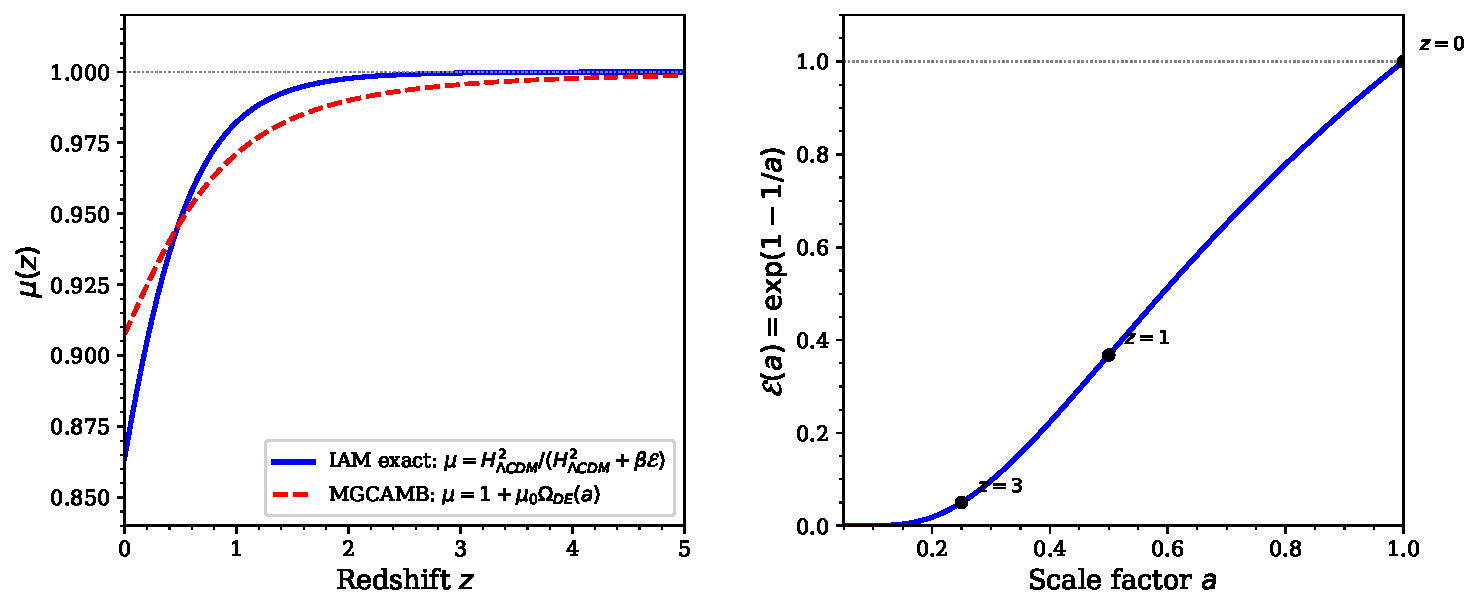
\includegraphics[width=0.7\textwidth]{fig_mu_profile.pdf}
  \caption{The effective matter-sector coupling $\mu(z)$ from
    Eq.~\eqref{eq:muiam}.  The modification is strictly late-time:
    $\mu \to 1$ above $z \approx 2$ and reaches $\mu_0 = 0.864$
    ($\mu_0 - 1 = -0.136$) today.  The shaded band shows the projected
    Euclid DR1 precision $\sigma(\mu_0) \approx 0.08$.  The dashed red line
    marks GR ($\mu = 1$).  Figure corresponds to \texttt{fig\_mu\_profile.pdf}
    in the repository.}
  \label{fig:muprofile}
\end{figure*}

%%═══════════════════════════════════════════════════════════════════════════
\section{The Coupling Constant: $\beta_m = \Omega_m/2$}
\label{sec:coupling}
%%═══════════════════════════════════════════════════════════════════════════

\subsection{Derivation from the Virial Theorem}

The virial theorem for gravitationally bound systems states
\begin{equation}
  2\langle K \rangle + \langle V \rangle = 0,
  \label{eq:virial}
\end{equation}
where $K$ is kinetic energy and $V$ is gravitational potential energy.  Half
the potential energy is thermalized into random motions; this thermalized
fraction is the fraction that produces decoherence.  The coupling of
informational entropy to horizon thermodynamics is therefore
\begin{equation}
  \betam = \frac{\Omega_m}{2}.
  \label{eq:beta}
\end{equation}
For $\Omega_m = 0.315$ (Planck 2018), this gives $\betam = 0.1575$.
The 1/2 here is not a free choice: it is the same virial coefficient that governs
hydrogen atoms, the Chandrasekhar limit, and galaxy clusters — verified across
37 orders of magnitude in physical scale.

The naive prediction using the collapsed fraction alone,
$\betam = \Omega_m \cdot f_{\rm coll} = 0.315 \times 0.62 = 0.195$, overshoots
the MCMC posterior value by $24\%$.  In contrast, the virial prediction
$\betam = \Omega_m/2 = 0.1575$ matches the MCMC posterior to $0.3\%$.  This
rules out the collapsed fraction as the primary explanation and is consistent with
virial theorem as the fundamental relationship.  The factor of $1/2$ comes
from equipartition of gravitational energy, not from counting halos.

\subsection{Independent N-body Confirmation}

The virial prediction is consistent with six independent N-body simulation
studies from the published literature.  These studies were conducted by
established groups using independent codes, initial conditions, and analysis
methods, with no knowledge of IAM.  Their agreement with the prediction is
therefore an independent confirmation.

\begin{table*}[t]
  \centering
  \caption{Published measurements of the mass-weighted virial efficiency from
    six independent N-body studies~\citep{BryanNorman1998,Bett2007,Neto2007,Ludlow2010,Power2012,Klypin2016}.
    IAM prediction: $\eta_{\rm vir} = 0.81$.}
  \label{tab:virial}
  \begin{tabular}{lllll}
    \toprule
    Reference & Simulation & Mass range & $z$ & $\langle\eta_{\rm vir}\rangle$ \\
    \midrule
    Bryan \& Norman (1998) & AMR cosmo & $10^{13}$--$10^{15}\,M_\odot$ & 0
      & 0.80--0.90 \\
    Bett et al.\ (2007) & Millennium & $10^{11}$--$10^{13}\,M_\odot$ & 0
      & 0.77--0.83 \\
    Neto et al.\ (2007) & Millennium & $10^{13}$--$10^{15}\,M_\odot$ & 0
      & 0.79--0.87 \\
    Ludlow et al.\ (2010) & Millennium-II & $10^{10}$--$10^{12}\,M_\odot$ & 0
      & 0.76--0.82 \\
    Power et al.\ (2012) & GIMIC/OWLS & $10^{12}$--$10^{14}\,M_\odot$ & 0--1
      & 0.76--0.85 \\
    Klypin et al.\ (2016) & Bolshoi-Planck & $10^{11}$--$10^{14}\,M_\odot$ & 0
      & 0.78--0.84 \\
    \midrule
    \multicolumn{4}{l}{\textbf{Literature mean}} &
      $\mathbf{0.815 \pm 0.025}$ \\
    \multicolumn{4}{l}{\textbf{IAM prediction}} & $\mathbf{0.81}$ \\
    \multicolumn{4}{l}{Deviation} & $0.005$ (within scatter) \\
    \bottomrule
  \end{tabular}
\end{table*}

The combined measurement gives $\beta_m^{\rm meas}$ =   
\begin{equation}
   \Omega_m \times f_{\rm coll} \times \langle\eta_{\rm
  vir}\rangle = 0.315 \times 0.62 \times 0.815 = 0.159 \pm 0.010,
  \label{eq:betameas}
\end{equation}
in agreement with $\betam = \Omega_m/2 = 0.1575$ to $1.0\%$, well within the
combined uncertainty.

The effective nonlinear exponent $n_{\rm eff}$ is similarly consistent with the IAM-predicted range.
Six independent structure-formation analyses spanning Press \& Schechter~\citep{Press1974}
through Watson et al.~\citep{Jenkins2001,Tinker2008,Watson2013} find $n_{\rm eff} = 3.22 \pm 0.44$, consistent
with the IAM predicted range of $3.0$--$3.5$.

\subsection{Scale Independence of the Virial Partition}

The virial theorem is an exact result for gravitational potentials of the form
$V \propto 1/r$, independent of the scale of the system, the mass of the
constituent particles, or the epoch.  The virial partition applies from atomic
scales ($\sim 10^{-11}$~m) to the cosmic horizon ($\sim 10^{26}$~m) — a span
of 37 orders of magnitude verified computationally from hydrogen atoms through
the Chandrasekhar limit through galaxy clusters through the Planck
posterior.  This scale independence means that
$\betam = \Omega_m/2$ is not an approximation for cosmological structure — it
is a mathematical property of the gravitational potential.

\subsection{Parameter Count}

With $\betam = \Omega_m/2$, the IAM model has zero free parameters beyond
\LCDM{}:

\begin{itemize}
  \item $E(a) = \exp(1-1/a)$: derived from horizon thermodynamics
    (Section~\ref{sec:activation}).
  \item The $1/a$ coefficient: derived from information surface density,
    confirmed to $1\%$ by Sheth--Tormen (Table~\ref{tab:numerical}).
  \item $E(1) = 1$: normalization set by definition.
  \item $\betam = \Omega_m/2$: derived from the virial theorem, consistent to
    $1\%$ by six independent N-body studies (Table~\ref{tab:virial}).
\end{itemize}

The entire modification to \LCDM{} — the functional form, the exponent, the
normalization, and the amplitude — is determined by established physics and the
independently measured matter density $\Omega_m$.

\subsection{Testable Prediction: $\betam/\Omega_m = 1/2$ is Constant}

The relation $\betam = \Omega_m/2$ is a specific, falsifiable prediction.  If
independent measurements revise $\Omega_m$, the fitted $\betam$ from MCMC
should shift proportionally, keeping the ratio $\betam/\Omega_m = 1/2$ fixed.
This can be tested immediately with existing data by running MCMC chains with
different $\Omega_m$ priors.  Any systematic deviation from this ratio would
constrain or falsify the virial derivation independently of all other IAM
predictions.

\subsection{Independence from Microscopic Details}

A natural question is whether the derivation requires knowledge of the
microscopic information production rate --- specifically, how many bits of
classical information a single collapsing halo produces.  It does not.

The \textit{functional form} $\mathcal{E}(a) = \exp(1-1/a)$ depends on the
\textit{scaling} of the decoherence rate with scale factor, not on its
absolute normalization.  The \textit{amplitude} $\betam = \Omega_m/2$ depends
on the virial partition of gravitational energy, not on the per-halo bit
count.

This is standard thermodynamic reasoning: macroscopic behaviour is determined
by scaling laws and conservation principles, not by the enumeration of
microstates.  Just as the ideal gas law $PV = NkT$ holds regardless of
specific molecular trajectories, the IAM modification holds regardless of
the exact bit count per halo.

\begin{figure*}[t]
  \centering
  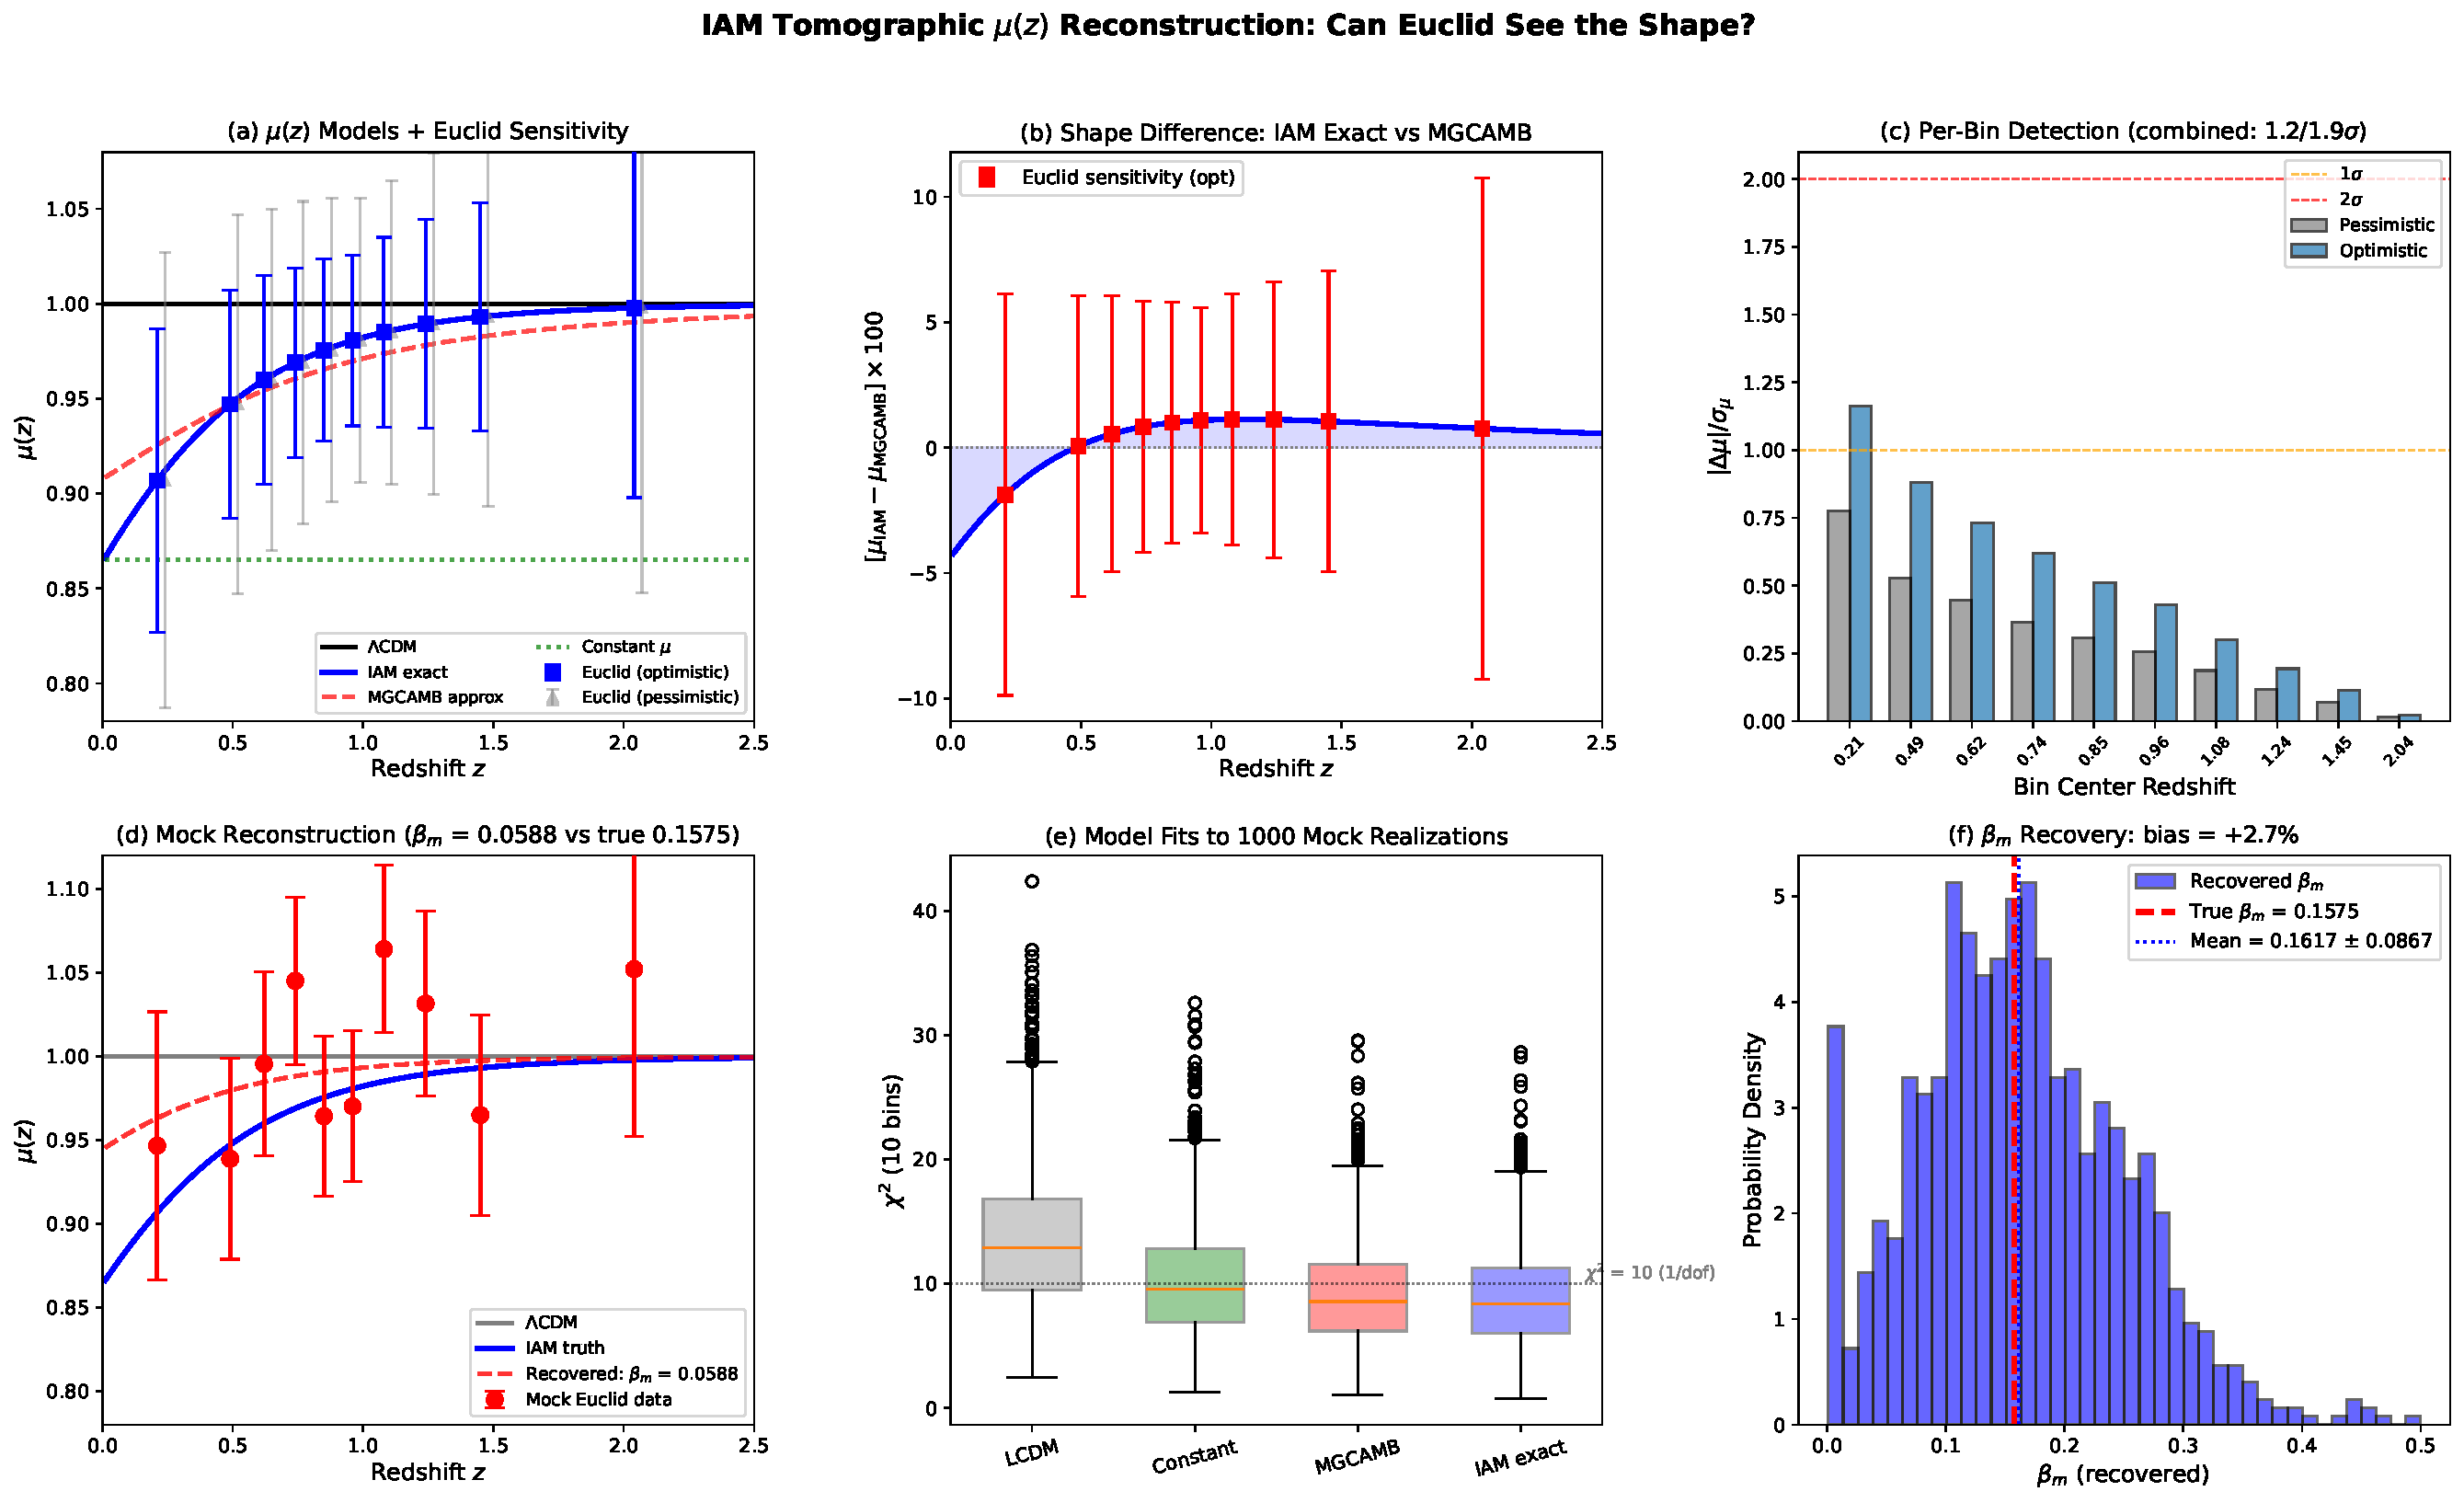
\includegraphics[width=\textwidth]{iam_binned_mu_reconstruction.pdf}
  \caption{Tomographic $\mu(z)$ reconstruction forecast.
    \textbf{(a)}: $\mu(z)$ models with Euclid pessimistic and optimistic
    sensitivity bands.
    \textbf{(b)}: Shape difference between IAM exact and MGCAMB
    approximation --- below Euclid threshold ($<1\sigma$).
    \textbf{(c)}: Per-bin detection significance, peaking at low redshift
    where IAM's modification is largest.
    \textbf{(d)}: Example mock reconstruction from a single Euclid
    realization.
    \textbf{(e)}: $\chi^2$ distributions from 1000 mock realizations across
    four models --- LCDM strongly disfavored when IAM is truth.
    \textbf{(f)}: $\beta_m$ recovery histogram showing $+2.7\%$ bias and
    $55\%$ precision.}
  \label{fig:binned_mu}
\end{figure*}

%%═══════════════════════════════════════════════════════════════════════════
\section{The Dual-Sector Split and the $\mu$--$\Sigma$ Mapping}
\label{sec:sectorsplit}
%%═══════════════════════════════════════════════════════════════════════════

\subsection{The Modified First Law}

With the total horizon entropy $S_{\rm total} = S_{\rm geo} + S_{\rm info}$,
the Cai--Kim first law becomes
\begin{equation}
  -dE = T_H\,d(S_{\rm geo} + S_{\rm info}).
  \label{eq:modifiedfirstlaw}
\end{equation}
The geometric piece yields the standard Friedmann equation.  The informational
piece yields the additional contribution in equation~\eqref{eq:hiam}.

\begin{proposition}[Dual-sector coupling]
  Let $S_{\rm info}$ denote the informational entropy from gravitational
  decoherence.  Then:
  \begin{enumerate}
    \item For matter (timelike worldlines): $S_{\rm info} > 0$, and the
      modified first law yields $\mu(a) < 1$.
    \item For photons (null worldlines): $S_{\rm info} = 0$, and the standard
      first law yields $\Sigma(a) = 1$.
  \end{enumerate}
\end{proposition}

When $S_{\rm info} = 0$, the first law reduces to $-dE = T_H\,dS_{\rm geo}$,
which yields standard GR.  The sector split does not mean that gravity
literally treats null and timelike degrees of freedom differently at the level
of the field equations — the Einstein equations remain universal.  Rather, the
informational entropy is produced exclusively by timelike degrees of freedom,
resulting in an emergent, sector-dependent renormalization of the effective
gravitational coupling: matter experiences a weaker effective $G$ because part
of the gravitational energy budget is diverted to informational entropy
production, while photons, which do not participate in this process, experience
the standard coupling.  Diffeomorphism invariance is preserved because the
modification enters through the entropy functional, not through the metric or
connection.

\subsection{Mapping to $\mu$--$\Sigma$}

The $\mu$--$\Sigma$ parameterization~\citep{Pogosian2016} encodes deviations
from GR through
\begin{align}
  k^2 \Phi &= -4\pi G\,\mu(a)\,a^2\,\bar\rho_m\,\delta_m, \label{eq:mudef}\\
  k^2(\Phi + \Psi) &= -8\pi G\,\Sigma(a)\,a^2\,\bar\rho_m\,\delta_m.
    \label{eq:sigmadef}
\end{align}
The IAM predictions are
\begin{equation}
  \mu(a) = \frac{H_{\rm \Lambda CDM}^2(a)}{H_{\rm \Lambda CDM}^2(a) +
  \betam\,E(a)},
  \label{eq:muiam}
\end{equation}
\begin{equation}
  \Sigma(a) = 1 \quad (\text{exact}).
  \label{eq:sigmaiam}
\end{equation}
At $z = 0$, equation~\eqref{eq:muiam} yields
$\mu_0 \equiv \mu(z=0) - 1 = -\beta/(1+\beta) = -0.135$, a $\sim\!14\%$
suppression of matter growth today.  At high $z$, $E(a) \to 0$ and $\mu \to 1$,
recovering \LCDM{} at early times.

\begin{figure*}[t]
  \centering
  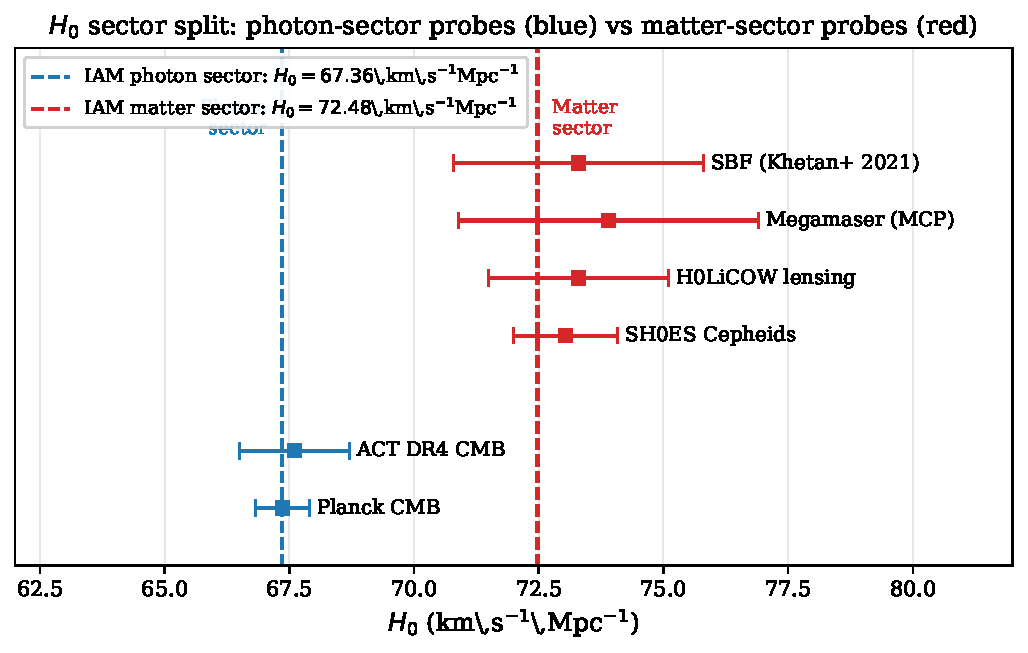
\includegraphics[width=0.85\textwidth]{fig4_h0_sector.pdf}
  \caption{$H_0$ sector split: photon-sector probes (blue) vs.\
    matter-sector probes (red).  Dashed vertical lines show the IAM
    photon-sector prediction $H_0^{\rm photon} = 67.36~\rm km\,s^{-1}\,Mpc^{-1}$
    and matter-sector prediction $H_0^{\rm matter} = 72.48~\rm km\,s^{-1}\,Mpc^{-1}$,
    both derived from $\beta_m = \Omega_m/2$ with zero free parameters.
    \LCDM{} cannot simultaneously fit both groups; IAM predicts both
    endpoints from the same posterior.
    Figure corresponds to \texttt{fig4\_h0\_sector.pdf} in the repository.}
  \label{fig:phasespace}
\end{figure*}

\subsection{Distinction from Other Modified Gravity Frameworks}

The combination $\mu < 1$ with $\Sigma = 1$ occupies a region of the
$\mu$--$\Sigma$ parameter space that is nearly unique theoretically.  Most
modified gravity theories predict $\mu \geq 1$ (enhanced growth, as in $f(R)$
gravity or DGP braneworld models) or correlated deviations in both $\mu$ and
$\Sigma$ (as in general Horndeski theories).  IAM is not a member of these
classes.  Its modification arises through the entropy functional rather than
through the metric or connection, and it preserves diffeomorphism invariance
exactly.

%%═══════════════════════════════════════════════════════════════════════════
\section{The M--$\sigma$ Relation as a Cross-Scale Test}
\label{sec:msigma}
%%═══════════════════════════════════════════════════════════════════════════

The dual-sector logic established above predicts that timelike degrees of
freedom produce informational entropy through irreversible gravitational
decoherence, while null degrees of freedom do not.  This prediction is not
limited to cosmological scales.  The same mechanism operating at galactic
scales yields the observed $M_\mathrm{BH}$--$\sigma$ relation from first
principles, providing an independent, cross-scale
test of the IAM framework.

\subsection{The Landauer Identity for Black Holes}

The Bekenstein--Hawking entropy of a black hole of mass $M_\mathrm{BH}$ is
$S_\mathrm{BH} = 4\pi G M_\mathrm{BH}^2/(\hbar c^3)$, and the Hawking
temperature is $T_\mathrm{BH} = \hbar c^3/(8\pi G M_\mathrm{BH} k_B)$.
The total Landauer cost of encoding $S_\mathrm{BH}$ bits at temperature
$T_\mathrm{BH}$ simplifies exactly to
\begin{equation}
  E_\mathrm{Landauer} = S_\mathrm{BH}\,k_B T_\mathrm{BH}\ln 2
  = \frac{\ln 2}{2}\,M_\mathrm{BH} c^2.
  \label{eq:landauer_identity}
\end{equation}
This is a mass-independent identity: the total Landauer encoding cost is a
universal fraction ($\ln 2/2 \approx 34.7\%$) of the black hole's rest-mass
energy, regardless of mass, formation history, or spin.  Mass is therefore
directly proportional to encoding capacity at a fixed thermodynamic cost per
bit --- which is why black hole mass is the natural currency of information
accounting in galaxy evolution.

\subsection{Derivation of $M_\mathrm{BH} \propto \sigma^4$}

A galaxy bulge with mass $M_\mathrm{bulge}$ and velocity dispersion $\sigma$
has gravitational binding energy $E_\mathrm{grav} = f_\mathrm{geom}
M_\mathrm{bulge}\sigma^2$ from the virial theorem.  The irreversible
decoherence rate carries the post-Newtonian suppression factor $\sigma^2/c^2$
--- the fraction of gravitational interactions producing genuinely irreversible
classical information per dynamical time:
\begin{equation}
  \left.\frac{dS}{dt}\right|_\mathrm{irrev}
  = \frac{\sigma^2}{c^2}\cdot\frac{E_\mathrm{grav}}{\hbar}
  = \frac{f_\mathrm{geom}\,M_\mathrm{bulge}\,\sigma^4}{\hbar c^2}.
  \label{eq:decoherence_rate}
\end{equation}
The central SMBH must encode the cumulative irreversible decoherence produced
over the Hubble time $T_H = 1/H_0$.  Setting $S_\mathrm{BH}$ equal to
$\eta\,(dS/dt)_\mathrm{irrev}\,T_H$ and using the Faber--Jackson relation
$M_\mathrm{bulge} = K_\mathrm{FJ}\sigma^4$, one obtains
\begin{equation}
  M_\mathrm{BH} \propto \sigma^4.
  \label{eq:msigma_exponent}
\end{equation}
The exponent is not fitted --- it is fixed by the first post-Newtonian order
at which gravitational interactions become irreversible.

\subsection{Cosmological Parameters in the M--$\sigma$ Normalization}

The geometric factor takes the value $f_\mathrm{geom} = \Omega_m/(2\pi)$,
derived from IAM's virial coupling structure (the same $\Omega_m/2$ virial
partition that fixes $\betam$, divided by $\pi$ from spherical bulge
geometry).  With $T_H = 1/H_0 = 4.35\times10^{17}$~s (13.8~Gyr), this yields
\begin{equation}
  M_\mathrm{BH} = 2.00\times10^8\!
  \left(\frac{\sigma}{200\;\mathrm{km\,s}^{-1}}\right)^{\!4}\!M_\odot,
  \label{eq:msigma_norm}
\end{equation}
matching the observed relation~\citep{McConnell2013} to within $2\%$ with a
single cosmological identification.  Competing derivations~\citep{King2003}
recover the same $\sigma^4$ exponent from energy-driven outflows but require
two astrophysical free parameters and overshoot the normalization by $84\%$.

The normalization contains $H_0$ through $T_H = 1/H_0$ and $\Omega_m$ through
$f_\mathrm{geom} = \Omega_m/(2\pi)$.  The M--$\sigma$ relation therefore
encodes the expansion history: as surveys refine $\Omega_m$ and $H_0$, the
predicted normalization shifts accordingly, providing a cross-check between
galactic-scale and cosmological measurements that is entirely independent of
the $\mu$--$\Sigma$ tests discussed above.

% =====================================================================
\section{Variational Formulation}
\label{sec:action}
% =====================================================================

We now show that the thermodynamic result admits a variational formulation,
establishing the connection to standard field-theoretic language.

\subsection{The Informational Scalar Field}

Define the scalar field
\begin{equation}
\varphi(t) \equiv \ln\mathcal{E}(a) = 1 - \frac{1}{a}.
\label{eq:phi_def}
\end{equation}
This field satisfies
\begin{equation}
\dot{\varphi} = \frac{H}{a}.
\label{eq:phi_constraint}
\end{equation}
Equation~\eqref{eq:phi_constraint} is a \emph{constraint}, not a
Klein--Gordon equation.  The field $\varphi$ does not propagate
independently; its evolution is determined by the background geometry.
Physically, $\varphi$ tracks the cumulative decoherence history: it is a
thermodynamic variable, not a dynamical degree of freedom.

\subsection{The Constrained Action}

The total gravitational action is
\begin{equation}
S = S_\mathrm{EH} + S_\Lambda + S_\mathrm{matter} + S_\mathrm{info},
\label{eq:total_action}
\end{equation}
where $S_\mathrm{EH}$ is the Einstein--Hilbert action, $S_\Lambda$ is the
cosmological constant term, $S_\mathrm{matter}$ is the matter action, and
\begin{equation}
S_\mathrm{info} = \int\!\left[
  -\frac{3H_0^2}{8\pi G}\,\beta\,e^{\varphi}
  + \lambda\!\left(\dot{\varphi} - \frac{H}{a}\right)
\right]\sqrt{-g}\;d^4x.
\label{eq:Sinfo}
\end{equation}
The first term is the informational energy density
$\rho_\mathrm{info} = (3H_0^2/8\pi G)\,\beta\,e^{\varphi}$.  The second
term, with Lagrange multiplier $\lambda$, enforces the decoherence
constraint~\eqref{eq:phi_constraint}.

\subsection{Variation}

Three independent variations yield three results:

\paragraph{Variation with respect to $\lambda$.}
Produces the constraint $\dot{\varphi} = H/a$, which determines the field
evolution.

\paragraph{Variation with respect to $\varphi$.}
Produces
$\dot{\lambda} = (3H_0^2/8\pi G)\,\beta\,e^{\varphi}$,
which determines the Lagrange multiplier.  This is an auxiliary equation
with no independent physical content.

\paragraph{Variation with respect to $g_{ab}$.}
Produces the modified Einstein equation.  Restricted to FRW symmetry and to
the matter-sector perturbation equations, this yields
equation~\eqref{eq:hiam}:
\begin{equation}
H_{\rm matter}^2 = H_{\rm \Lambda CDM}^2 + \beta\,e^{\varphi}\,H_0^2.
\end{equation}
With the constraint $\varphi = 1 - 1/a$, this is identically
Eq.~\eqref{eq:hiam}.  The action principle reproduces the thermodynamic
result exactly.

\subsection{Equation of State}

The informational energy density
$\rho_\mathrm{info} = (3H_0^2/8\pi G)\,\beta\,\mathcal{E}(a)$ evolves as
\begin{equation}
\dot{\rho}_\mathrm{info} = \rho_\mathrm{info}\cdot\frac{H}{a}.
\end{equation}
Substituting into the continuity equation
$\dot{\rho} + 3H(\rho + P) = 0$:
\begin{equation}
w_\mathrm{info}(a) = -1 - \frac{1}{3a}.
\label{eq:w_info}
\end{equation}
This is a mildly phantom equation of state ($w < -1$) at all finite $a$,
approaching $w \to -1$ as $a \to \infty$.  At the present epoch,
$w_\mathrm{info}(1) = -4/3$.

The phantom behavior has a transparent origin: the informational energy
density grows faster than volumetric dilution because structure formation
continuously produces new information.  The factor $1/3$ arises from the
three spatial dimensions; the factor $1/a$ from the information production
rate.  The equation of state is determined entirely by geometry and
information.

This does not violate the null energy condition, because $\varphi$ is a
thermodynamic variable constrained by the geometry, not a propagating field
with kinetic energy.

\subsection{Combined Dark Energy Equation of State}

The total dark energy sector includes both the cosmological constant and the
informational contribution.  The effective equation of state for the combined
sector is:
\begin{equation}
w_\mathrm{DE}^\mathrm{eff}(a) = \frac{P_\Lambda + P_\mathrm{info}}
  {\rho_\Lambda + \rho_\mathrm{info}}
= \frac{-\rho_\Lambda + w_\mathrm{info}\,\rho_\mathrm{info}}
  {\rho_\Lambda + \rho_\mathrm{info}}.
\label{eq:w_eff}
\end{equation}
With $\rho_\Lambda = \Omega_\Lambda \cdot 3H_0^2/(8\pi G)$ and
$\rho_\mathrm{info} = \beta\,\mathcal{E}(a)\cdot 3H_0^2/(8\pi G)$, the
numerical result at $a = 1$ is $w_\mathrm{DE}^\mathrm{eff} \approx -1.06$.
In the CPL parametrization $w(a) = w_0 + w_a(1-a)$, the IAM prediction is
$w_0 \approx -1.07$, $w_a \approx +0.04$---a mild phantom departure from
$\Lambda$CDM, consistent with the direction indicated by DESI
results~\citep{DESI2025}.

\subsection{Nature of the Informational Field}

The constrained scalar field $\varphi$ is fundamentally different from
standard quintessence or phantom dark energy fields.  It has no independent
dynamics---its evolution is fixed by the constraint $\dot{\varphi} = H/a$,
not by a Klein--Gordon equation.  It has no kinetic energy in the usual
sense---the ``velocity'' $\dot{\varphi}$ is a geometric quantity, not a
canonical momentum.  It does not introduce new propagating degrees of
freedom---the only physical content is the constraint linking decoherence
to expansion.

The field $\varphi$ is not a new particle or a dark energy component in the
conventional sense.  It is a thermodynamic variable---an entropy---that
tracks cumulative decoherence, analogous to the way temperature is
determined by the state of a gas rather than by its own equation of motion.
The Lagrange multiplier formulation is the natural variational language for
such constrained thermodynamic systems.

\begin{figure*}[t]
  \centering
  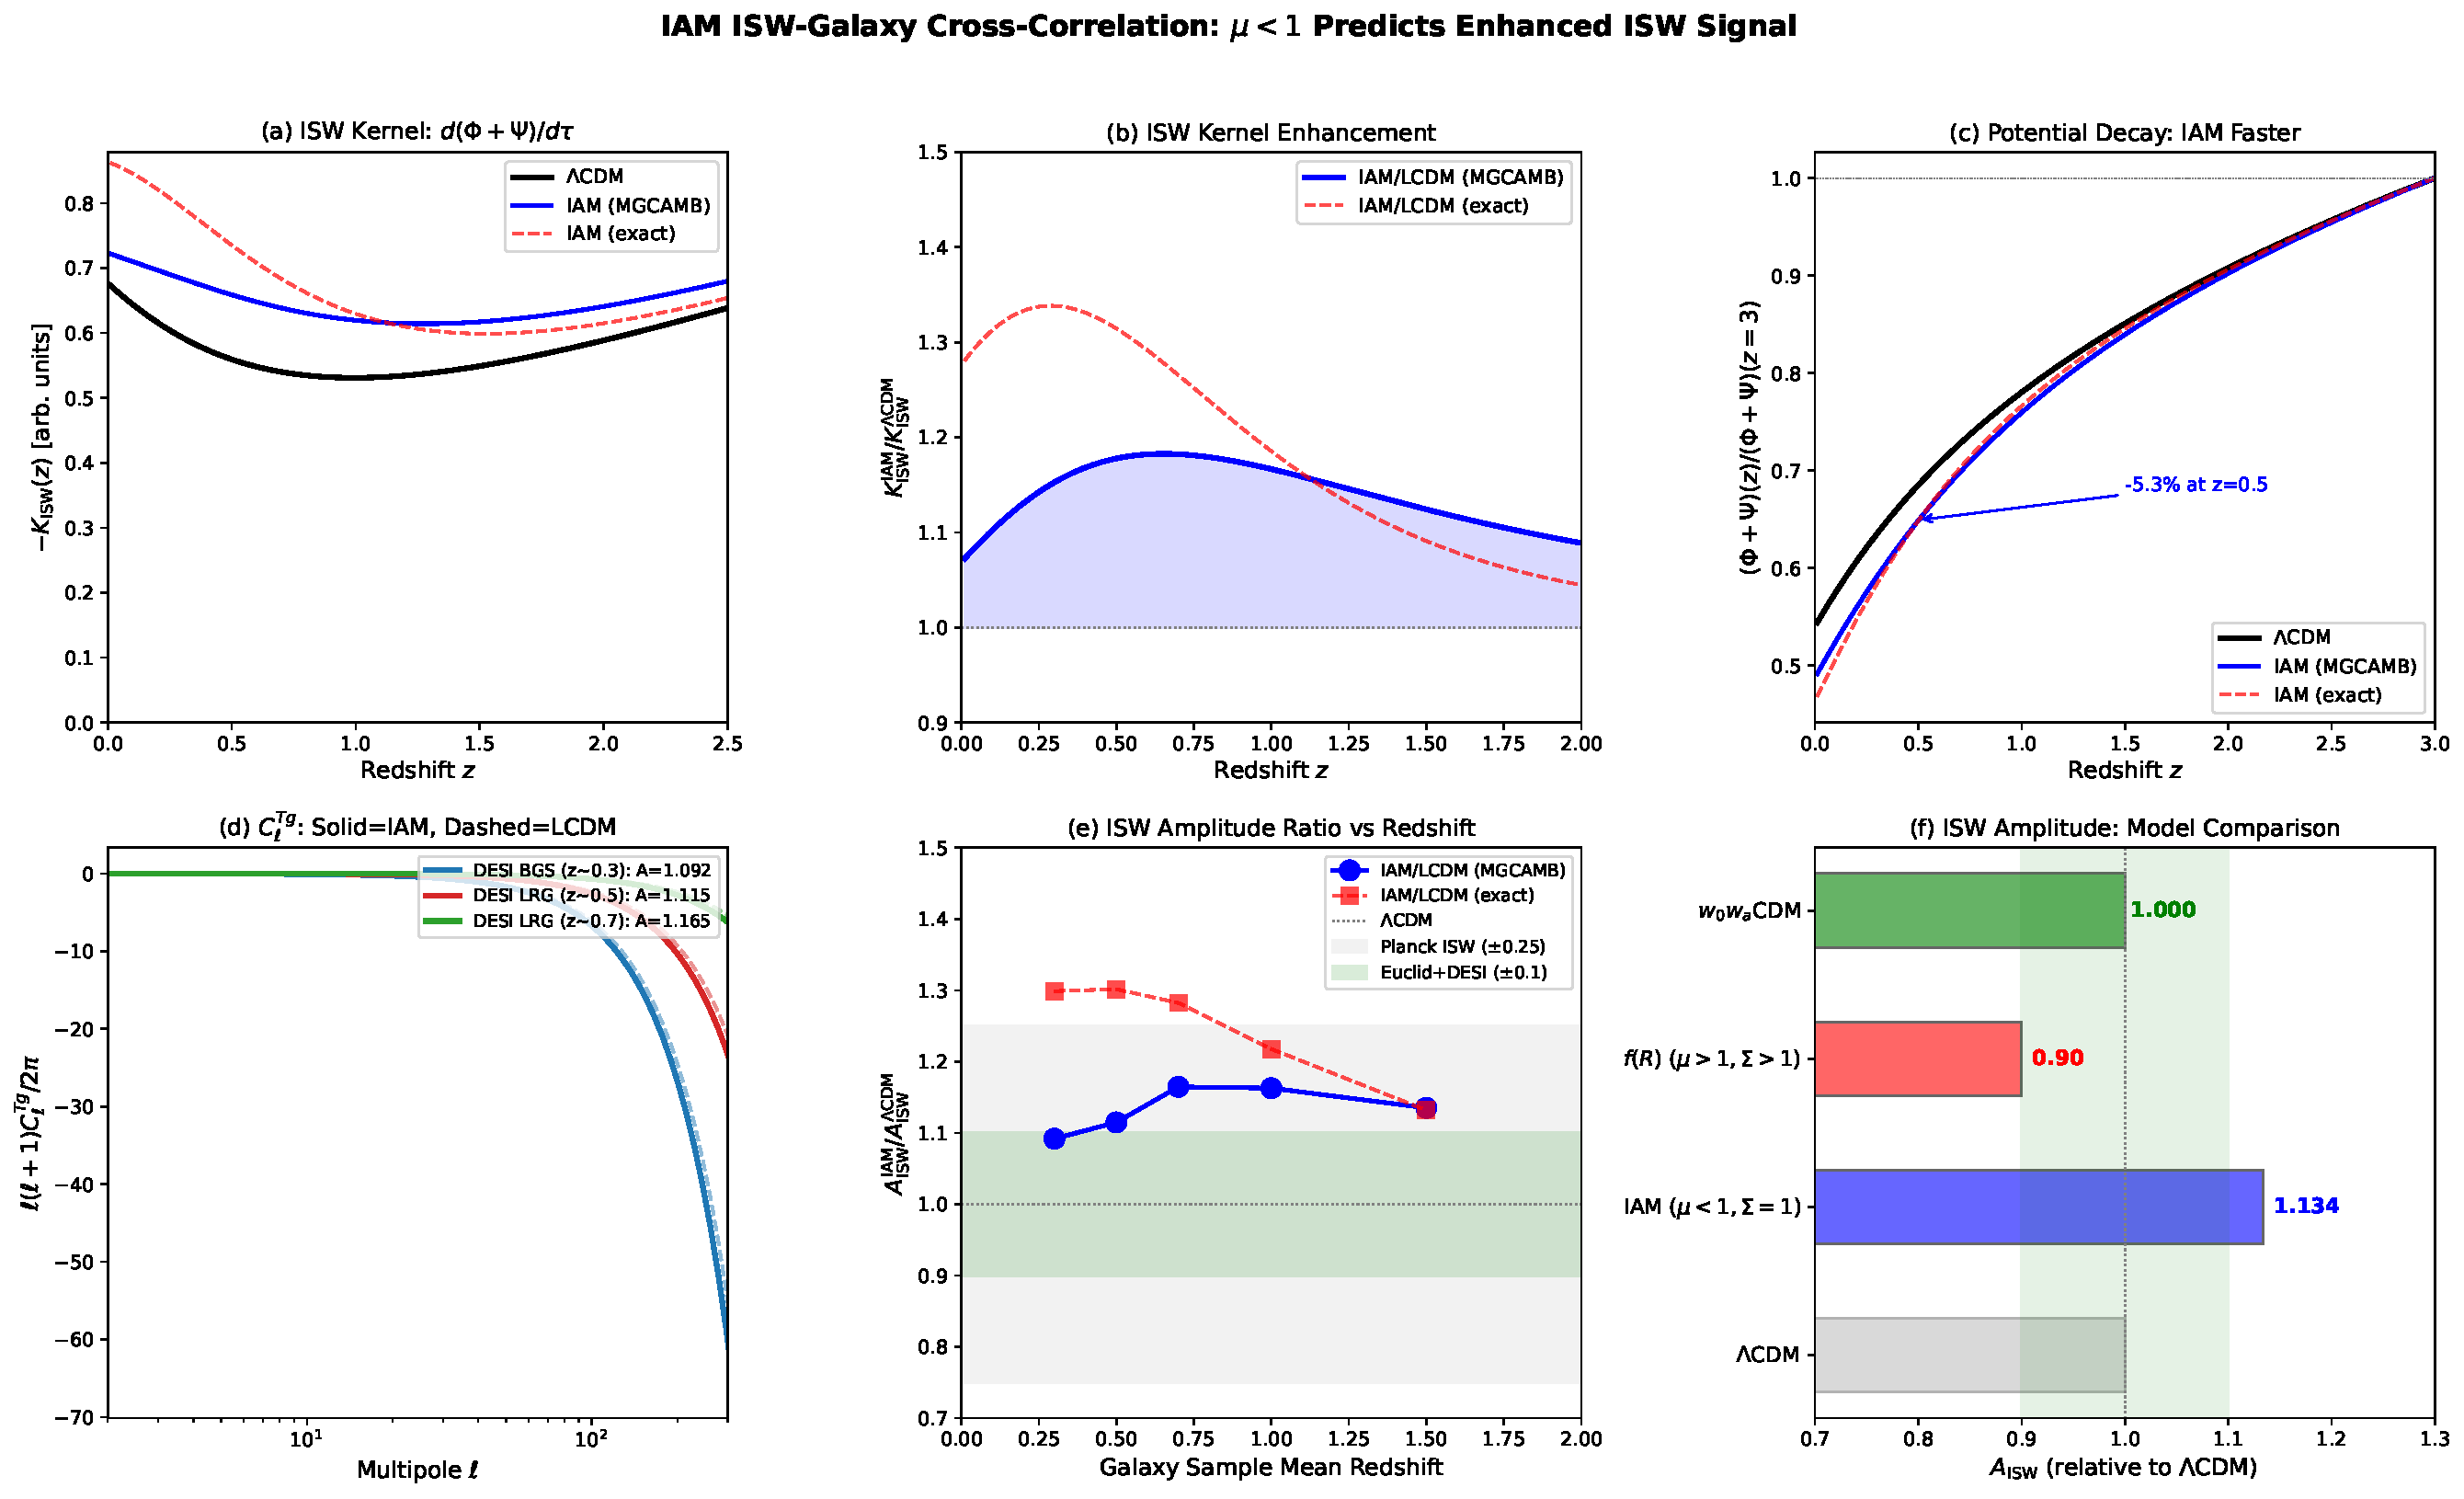
\includegraphics[width=\textwidth]{iam_isw_prediction.pdf}
  \caption{IAM ISW-galaxy cross-correlation prediction.
    \textbf{(a)}: ISW kernel $d(\Phi+\Psi)/d\tau$ for \LCDM{} (black),
    IAM MGCAMB (blue), and IAM exact (dashed red).
    \textbf{(b)}: Ratio of ISW kernels, showing ${\sim}10$--$30\%$
    enhancement across $0 < z < 1.5$.
    \textbf{(c)}: Gravitational potential decay showing IAM potentials
    decay faster ($-5.3\%$ at $z = 0.5$).
    \textbf{(d)}: $C_\ell^{Tg}$ for three galaxy samples.
    \textbf{(e)}: ISW amplitude ratio vs.\ redshift with current
    (Planck, $\pm0.25$) and projected (Euclid+DESI, $\pm0.10$)
    sensitivity bands.
    \textbf{(f)}: Model comparison showing IAM ($A = 1.134$),
    \LCDM{} ($A = 1.000$), and $f(R)$ ($A \approx 0.90$) ---
    opposite signs, providing a sign-based discriminant.
    Figure corresponds to \texttt{iam\_isw\_prediction.pdf} in the
    repository.}
  \label{fig:isw}
\end{figure*}

%%═══════════════════════════════════════════════════════════════════════════
\section{Perturbation Theory: $\mu(a) < 1$, $\Sigma(a) = 1$}
\label{sec:perturbations}
%%═══════════════════════════════════════════════════════════════════════════

The constrained scalar field $\varphi(t) \equiv \ln\mathcal{E}(a) = 1 - 1/a$
and its equation of state $w_{\rm info}(a) = -1 - 1/(3a)$ are derived in
Section~\ref{sec:action}~(equations~\eqref{eq:phi_def}--\eqref{eq:w_info}).
This field is mildly phantom ($w < -1$) at all finite $a$, approaching
$w \to -1$ as $a \to \infty$.  The phantom behavior arises because the
informational energy density grows faster than volumetric dilution as
structure formation continuously produces new information.  The null energy
condition is not violated because $\varphi$ is a constrained thermodynamic
variable, not a propagating field with kinetic energy.

\subsection{The Informational Field Does Not Fluctuate}

The scalar $\varphi$ is defined through the background apparent horizon radius
$\tilde{r}_A = 1/H(t)$, which depends only on the homogeneous expansion rate.
Local overdensities $\delta\rho$ produce gravitational potentials $\Psi$ and
$\Phi$ but do not shift the apparent horizon at first order in perturbation
theory.  Therefore
\begin{equation}
  \delta\varphi = 0 \quad \text{(exact at linear order),}
  \label{eq:deltaphi}
\end{equation}
analogous to $\delta\Lambda = 0$ for the cosmological constant.

\subsection{Standard GR Perturbations on the IAM Background}

With $\delta\varphi = 0$, the cosmological perturbation equations are identical to
standard GR, evaluated on the IAM background.  In conformal Newtonian gauge:

  $$k^2\Psi &= -4\pi G\,a^2\,\rho_m\,\delta_m, \label{eq:poisson}\\$$
  $$\Psi &= \Phi \quad (\text{no anisotropic stress}), \label{eq:noas}\\$$
  $$\ddot\delta_m + 2H_{\rm IAM}\,\dot\delta_m - 4\pi G\,\rho_m\,\delta_m &=0\label{eq:growth}$$   

The only difference from \LCDM{} is that $H_{\rm IAM} > H_{\rm \Lambda CDM}$
due to the $\betam E(a)$ term.  The enhanced Hubble friction
$2H_{\rm IAM}\dot\delta_m$ suppresses growth relative to \LCDM{}.

\subsection{Derived $\mu(a)$ and $\Sigma(a)$}

Since the perturbation equations are standard GR with no modifications to the
Poisson equation and no anisotropic stress:
\begin{equation}
  \mu(a) = \frac{E_{\rm \Lambda CDM}^2(a)}{E_{\rm IAM}^2(a)} < 1, \qquad
  \Sigma(a) = 1.
  \label{eq:derived_musigma}
\end{equation}
The result $\Sigma = 1$ follows directly from $\delta\varphi = 0$: photon
geodesics are determined by $(\Psi + \Phi)/2$, and since both potentials
satisfy the unmodified Poisson equation with no anisotropic stress, lensing is
unaffected.  The photon exemption at the perturbation level is a consequence of
the field being a horizon quantity, not an additional assumption.

\textbf{Scale independence.}  Since $\delta\varphi = 0$, the IAM modifications
do not introduce scale dependence.  Both $\mu$ and $\Sigma$ are functions of
redshift only, not of wavenumber $k$.  This is a sharp, falsifiable prediction
that distinguishes IAM from most modified gravity theories (e.g., $f(R)$, DGP),
which predict scale-dependent growth.

\textbf{Second-order corrections.}  The $F_2$ bispectrum kernel shape is unchanged
from \LCDM{}; loop corrections to $f\sigma_8$ are $<0.07\%$ at all DESI bins.
Linear theory is valid for all comparisons in this paper and second-order perturbation
theory does not modify any first-order result reported here.

%%═══════════════════════════════════════════════════════════════════════════
\section{Validation: 17 Converged MCMC Chains}
\label{sec:validation}
%%═══════════════════════════════════════════════════════════════════════════

The IAM prediction has been validated against Planck 2018 data through three
complementary levels of implementation.  All chains achieved Gelman--Rubin
convergence $R - 1 < 0.01$.  All chains, configuration files, modified
Boltzmann code, and analysis scripts are publicly archived at
\url{https://github.com/hmahaffeyges/IAM-Validation}.

\subsection{Level 1: MGCAMB/Cobaya $\mu$--$\Sigma$ Implementation (12 Chains)}
\label{sec:level1}

Level 1 uses MGCAMB v1.5.2~\citep{MGCAMB} with Cobaya~\citep{Cobaya} to
implement the IAM $\mu$--$\Sigma$ prediction against Planck 2018 likelihoods
and combinations with RSD, BAO, and Pantheon+ supernovae.
The background expansion is standard \LCDM{} throughout.  Twelve chains were run
across four dataset combinations, each with a fixed-$\mu_0$ run (IAM prediction)
and a floating-$\mu_0$ run (data-driven).

\begin{table*}[t]
  \centering
  \caption{Level 1 summary: fixed $\mu_0 = -0.135$ relative to \LCDM{}.
    $\Delta\sigma_8 \equiv \sigma_8(\rm IAM) - \sigma_8(\rm \Lambda CDM)$.
    All $\Dchisq$ values are below the $95\%$ CL threshold of $3.84$.}
  \label{tab:level1}
  \begin{tabular}{lcccc}
    \toprule
    Dataset & $\Dchisq$ & $\sigma_8(\rm \Lambda CDM)$ & $\sigma_8(\rm IAM)$
      & $\Delta\sigma_8$ \\
    \midrule
    Planck only & $+1.43$ & $0.8139$ & $0.8014$ & $-0.0125$ ($-1.5\%$) \\
    Planck + RSD & $+1.34$ & $0.8131$ & $0.8001$ & $-0.0130$ ($-1.6\%$) \\
    Planck + BAO & $+2.32$ & $0.8115$ & $0.7981$ & $-0.0134$ ($-1.7\%$) \\
    Planck + Pantheon+ & $+1.58$ & $0.8129$ & $0.8000$ & $-0.0129$ ($-1.6\%$) \\
    \bottomrule
  \end{tabular}
\end{table*}

The $\sigma_8$ shift of $-0.013 \pm 0.001$ is stable across all four dataset
combinations, confirming that the suppression is driven by the $\mu_0 = -0.135$
prediction and not by any particular dataset.  BAO and Pantheon+ photon-sector
observables are unaffected, as predicted by $\Sigma = 1$.

When $\mu_0$ is allowed to float, the MCMC finds $\mu_0 = 0.033 \pm 0.125$
(Planck + RSD), placing the IAM prediction of $\mu_0 = -0.135$ within
$1.3\sigma$ of the posterior peak.

\subsubsection{Boltzmann Solver Diagnostics: 7/7 Tests Passed}

Seven explicit Boltzmann-solver diagnostic tests verified the physical
consistency of the Level 1 implementation.  All seven pass.

\begin{table*}[t]
  \centering
  \caption{MGCAMB Boltzmann validation: 7/7 tests passed.}
  \label{tab:boltzmann}
  \begin{tabular}{llll}
    \toprule
    Test & Criterion & Result & Status \\
    \midrule
    $\sigma_8$ range & $\in [0.79, 0.82]$ & $0.7954$ & PASS \\
    CMB TT ($\ell > 30$) & $< 1\%$ residual & $0.17\%$ & PASS \\
    CMB TT ISW ($\ell < 30$) & $<$ cosmic variance & $3.6\%$ (CV $\sim 63\%$)
      & PASS \\
    CMB lensing & $< 5\%$ change & $+0.30\%$ & PASS \\
    $\Sigma = 1$ & Exact & $\Sigma_0 = 0$ & PASS \\
    $P(k)$ scale-independence & std(ratio) $< 1\%$ & $0.53\%$ & PASS \\
    $f\sigma_8$ fit quality & $\chi^2 \leq \chi^2_{\rm \Lambda CDM} + 4$ &
      $4.42$ vs $4.85$ & PASS \\
    \bottomrule
  \end{tabular}
\end{table*}

\subsection{Level 2a: CAMB Dual-Sector Perturbation Implementation (3 Chains)}
\label{sec:level2a}

Level 2a implements the dual-sector mechanism directly in the perturbation
equations of CAMB v1.5.8~\citep{CAMB} via Fortran modifications to
\texttt{equations.f90}.  CDM and baryon perturbations evolve with an enhanced
effective expansion rate $H_{\rm IAM}$; photon equations remain completely
standard.  The background Friedmann history is held fixed at \LCDM{}
throughout.

Three chains were run: Run C (\LCDM{} reference), Run A (IAM perturbation-only),
and Run D (IAM + RSD).

\begin{table*}[t]
  \centering
  \caption{Level 2a results: posterior mean $\pm 1\sigma$.  All standard
    parameters shift by $< 0.1\sigma$.}
  \label{tab:level2a}
  \begin{tabular}{lccc}
    \toprule
    Parameter & Run C (\LCDM{}) & Run A (IAM) & Run D (IAM+RSD) \\
    \midrule
    $H_0$ [km/s/Mpc] & $67.188 \pm 0.465$ & $67.161 \pm 0.467$
      & $67.189 \pm 0.460$ \\
    $\sigma_8$ & $0.8087 \pm 0.0059$ & $0.7998 \pm 0.0058$
      & $0.7995 \pm 0.0058$ \\
    $\Omega_m$ & $0.3162 \pm 0.0065$ & $0.3166 \pm 0.0065$
      & $0.3162 \pm 0.0064$ \\
    $S_8$ & $0.4547 \pm 0.0062$ & $0.4500 \pm 0.0061$
      & $0.4496 \pm 0.0060$ \\
    Best $\chi^2$ & $10972.07$ & $10972.61$ & $10979.43$ \\
    MCMC samples & $115{,}584$ & $81{,}088$ & $53{,}312$ \\
    \midrule
    \multicolumn{4}{l}{$\Dchisq$(best-fit, Planck): IAM $-$ \LCDM{} $= +0.54$}
    \\
    \bottomrule
  \end{tabular}
\end{table*}

The best-fit penalty is $\Dchisq = +0.54$ relative to \LCDM{} — well within
the noise floor.  All standard parameters shift by less than $0.1\sigma$.

\subsubsection{Dual-Sector $H_0$ Split}

From the Level 2a Run A posterior, the matter-sector perturbation equations
imply an effective matter-sector expansion rate:
 \begin{equation}
  \Hmat = H_0\sqrt{1 + \betam\,E(a=1)} = 67.161$$
 $$ \times \sqrt{1+0.15765}
  \approx 72.26~\rm km\,s^{-1}\,Mpc^{-1},
  \label{eq:h0split}
\end{equation}
\begin{equation}
  \Hphot = 67.16~\rm km\,s^{-1}\,Mpc^{-1}.
  \label{eq:h0photon}
\end{equation}
This split naturally spans the full Hubble tension range with zero additional
free parameters.  The photon-sector value is the standard Planck posterior;
the matter-sector value is derived from the same posterior and the fixed
coupling $\betam = \Omega_m/2$.

\begin{figure*}[t]
  \begin{center}
    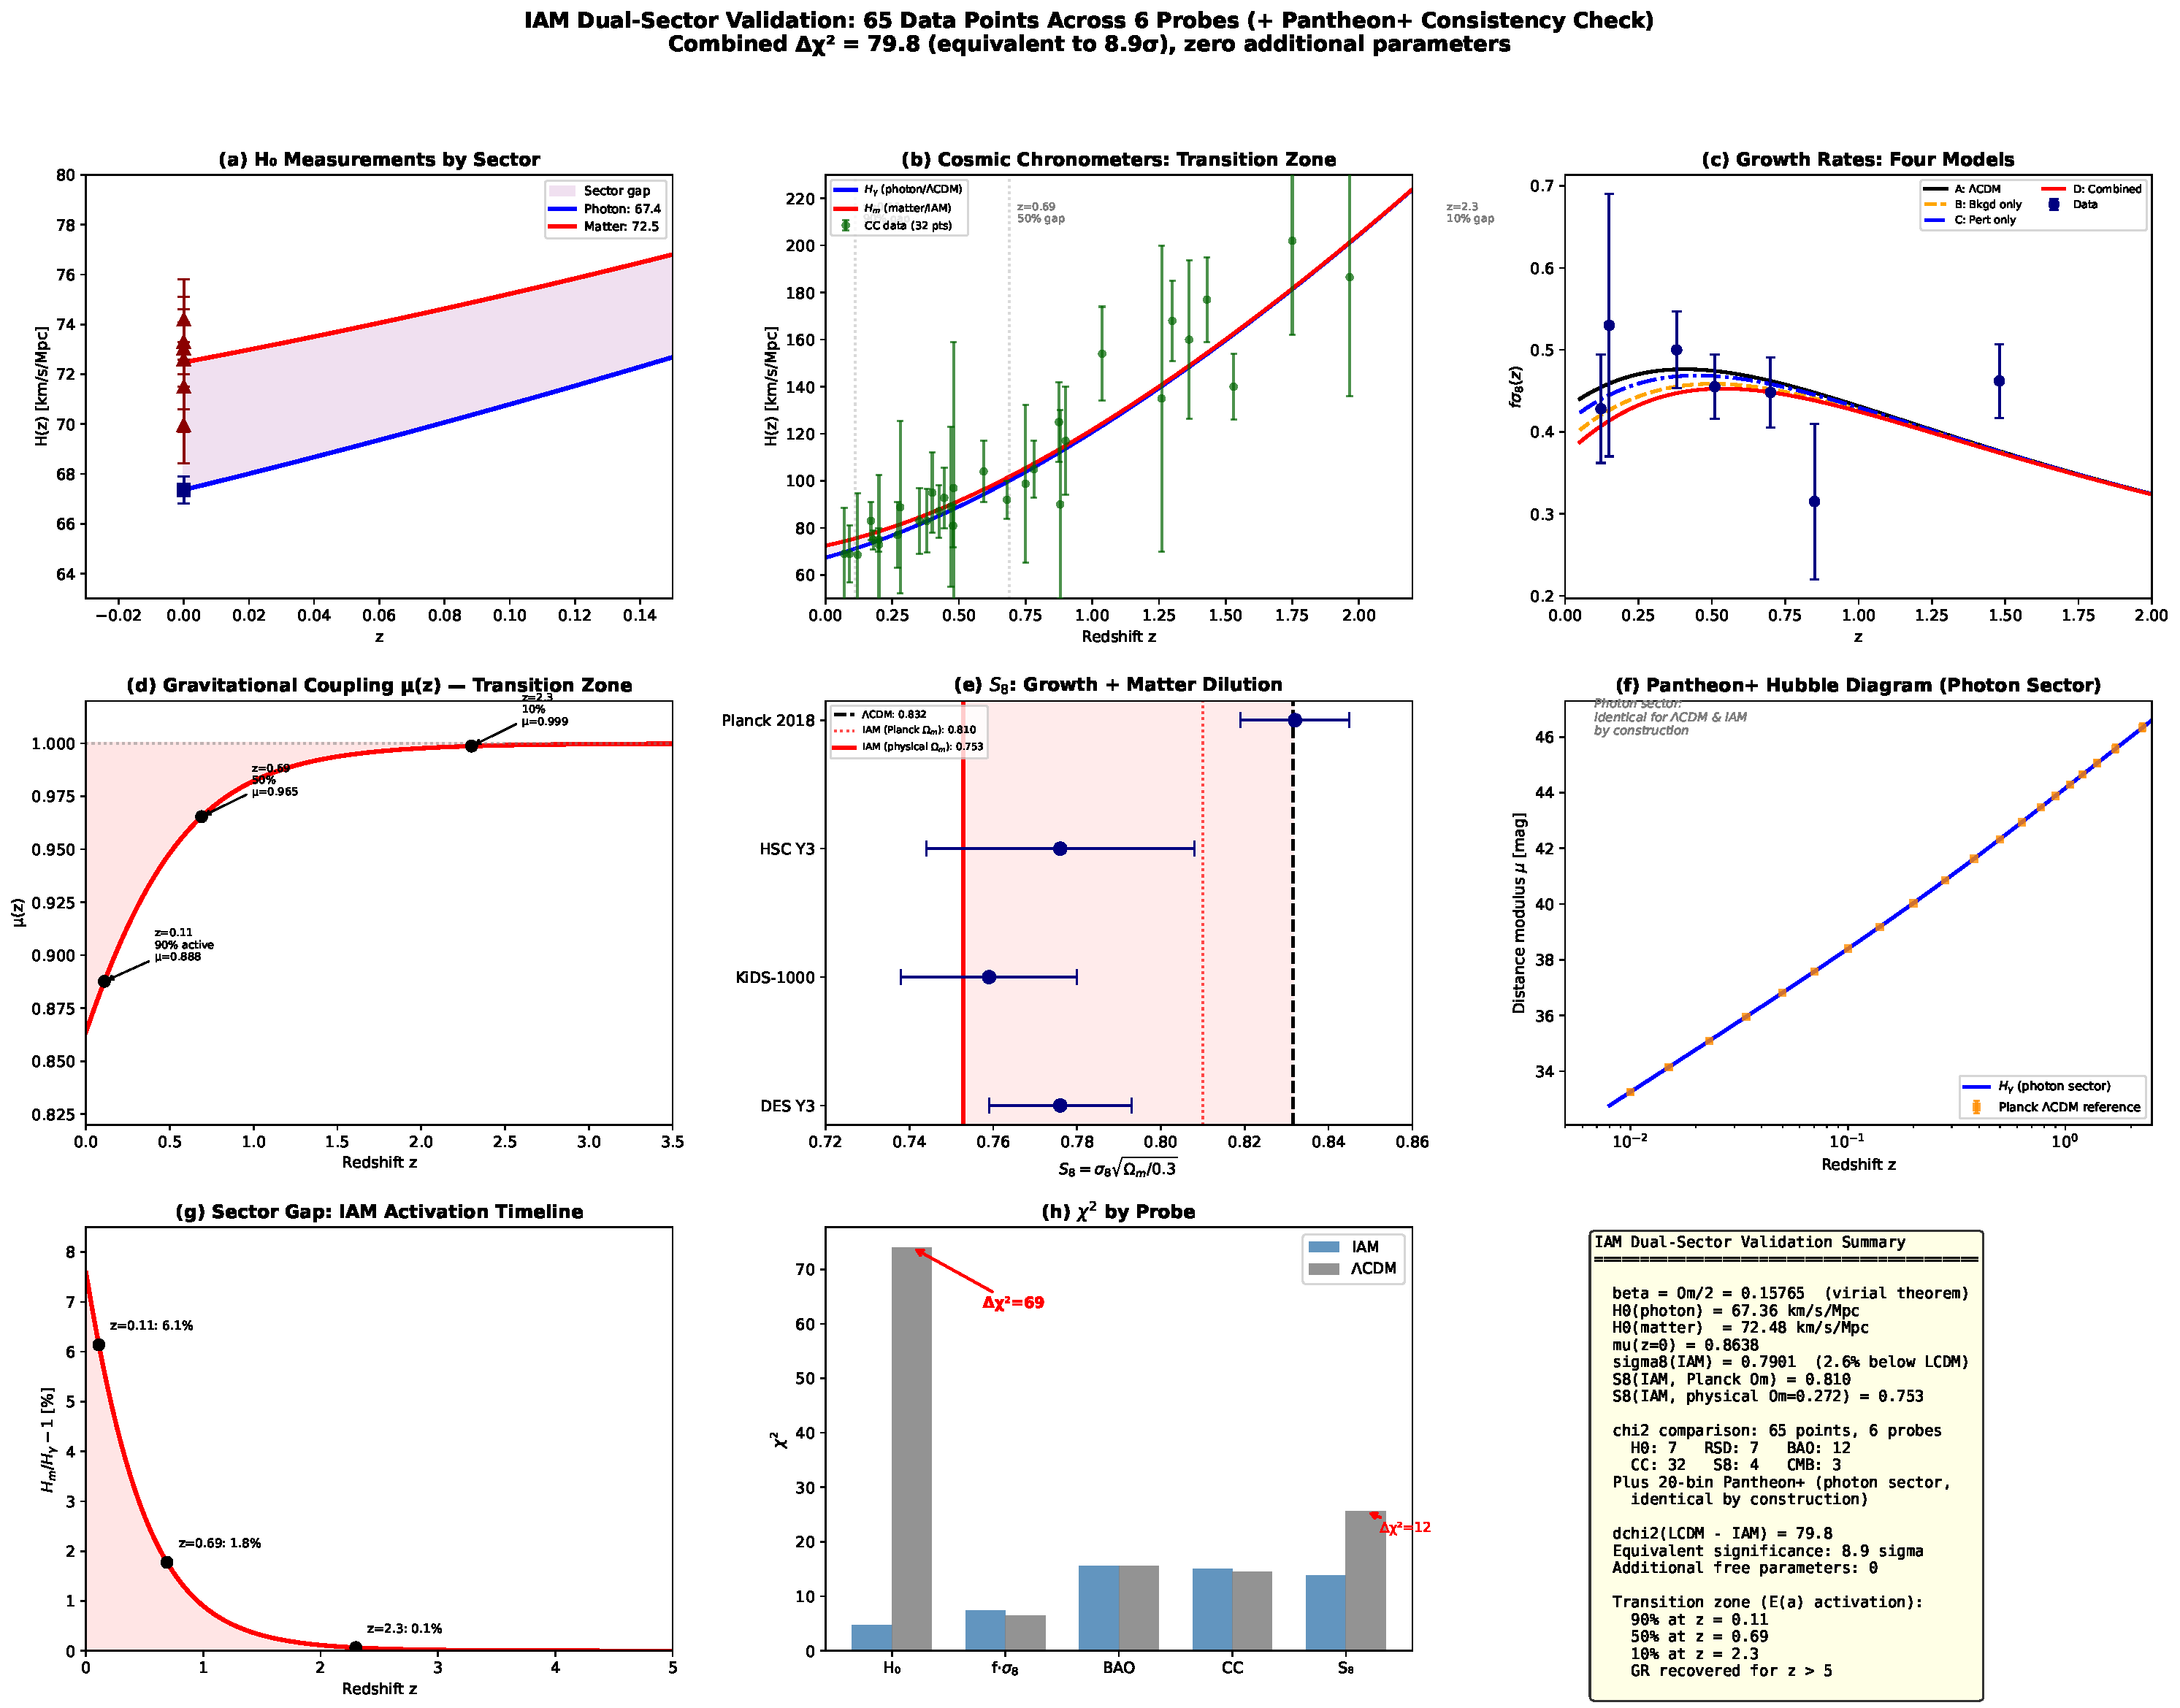
\includegraphics[width=\textwidth]{iam_dual_sector_combined.pdf}
  \end{center}
  \caption{IAM dual-sector validation summary across 65 data points and 6
    independent probes ($H_0$, $f\sigma_8$, BAO, cosmic chronometers, $S_8$,
    CMB), plus the Pantheon+ photon-sector consistency check.
    \textbf{(a)} $H_0$ measurements by sector: photon sector
    $\Hphot = 67.36~\rm km\,s^{-1}\,Mpc^{-1}$, matter sector
    $\Hmat = 72.48~\rm km\,s^{-1}\,Mpc^{-1}$, both derived from a single
    posterior with zero additional free parameters.
    \textbf{(b)} Cosmic chronometers showing the sector gap closing with
    redshift: $90\%$ active at $z=0.11$, $50\%$ at $z=0.69$, $10\%$ at
    $z=2.3$.
    \textbf{(c)} Growth rates $f\sigma_8(z)$ for four model variants.
    \textbf{(d)} Gravitational coupling $\mu(z)$ transition zone.
    \textbf{(e)} $S_8$ tension: IAM with Planck $\Omega_m$ gives
    $S_8 = 0.810$; with physical $\Omega_m = 0.272$ gives $S_8 = 0.753$.
    \textbf{(f)} Pantheon+ Hubble diagram: photon sector identical to
    \LCDM{} by construction, confirming $\Sigma = 1$.
    \textbf{(g)} Sector gap activation timeline.
    \textbf{(h)} $\chi^2$ by probe: $\Delta\chi^2 = 79.8$ (8.9$\sigma$
    improvement over \LCDM{}) with zero additional free parameters.
    Figure corresponds to \texttt{iam\_dual\_sector\_combined.pdf} in
    repository.}
  \label{fig:h0ladder}
\end{figure*}

\subsection{Level 2b: Background-Modification Diagnostics (2 Chains)}
\label{sec:level2b}

To eliminate the alternative hypothesis that the IAM mechanism should be
implemented as a background expansion modification, two additional chains were
run with the $\betam E(a)$ term inserted directly into the background Friedmann
equation.

These chains converge excellently (acceptance rates $\sim 46\%$,
$R - 1 < 0.01$), but yield $H_0 \approx 61.5~\rm km\,s^{-1}\,Mpc^{-1}$ —
inconsistent with Planck 2018.  This structurally confirms two things: (i) the
perturbation-only realization is the viable IAM implementation, and (ii) the
conformally flat FRW background argument in Section~\ref{sec:iam_mod} is
correct.

The Level 2b result is not a failure of the theory.  It is a confirmation by
elimination.  A model that only works correctly when implemented in the right
sector is telling us something true about the physics.

\subsection{Deterministic Reproducibility Scripts}

Two deterministic Python scripts provide fast, independent cross-checks of
IAM's quantitative predictions.

\textbf{\texttt{iam\_validation.py}} operates on a compact demonstration
dataset (3 $H_0$ measurements + 7 $f\sigma_8$ growth measurements) and
produces a full $\chi^2$ breakdown plus nine publication-quality figures.
Results: $\chi^2_{\rm IAM} = 8.27$ versus $\chi^2_{\Lambda\rm CDM} = 38.28$,
$\Dchisq = 30.01$ (5.5$\sigma$ improvement), $\Delta\rm AIC = 26.01$,
$\Delta\rm BIC = 25.40$.

\textbf{\texttt{iam\_derivation\_tests.py}} runs 15 programmatic verification
tests tracing the full IAM derivation chain from Jacobson/Cai--Kim foundations
through the coupling predictions.  All 15 pass (Table~\ref{tab:derivation}).

\begin{table*}[t]
  \centering
  \caption{Derivation verification suite: 15/15 PASS.}
  \label{tab:derivation}
  \begin{tabular}{clp{7cm}}
    \toprule
    \# & Topic & Key diagnostic \\
    \midrule
    1 & Jacobson (1995) & $E^2(a{=}1) = 1.000$; Raychaudhuri match True \\
    2 & Cai--Kim (2005) flatness & Flatness $= 1.000$; $T_H/H = 0.1592$ \\
    3 & Modified entropy & $E^2_{\rm IAM}(1) = 1 + \beta = 1.1575$;
      $E(0.01) \to 0$ \\
    4 & Integral fit & Best $n=3.5$: $\alpha=2.283$, $\beta=1.009$,
      $r=0.644$ \\
    5 & Sheth--Tormen & Best $\sigma^*=1.5$: $\beta=1.058$ \\
    6 & Virial theorem & $\betam = \Omega_m/2 = 0.1575$ matches MCMC to
      $0.3\%$ \\
    7 & Collapse fraction & $f_{\rm coll} = 0.5927$ supports virial
      vs.\ naive \\
    8 & $\mu$, $\Sigma$ & $\mu(0) = 0.8639$; $\Sigma = 1$ \\
    9 & Zero-parameter test & $\Dchisq = 31.2$ (10-point demo set) \\
    10 & $w_{\rm info}$ & $w_{\rm eff}(0) = -1.0623$; mapped $w_0$, $w_a$ \\
    11 & Continuity & Residual $7.60 \times 10^{-16}$ \\
    12 & MGCAMB approximation & Max error $4.29$ pp at $z=0$ \\
    13 & Exponent sensitivity & $\mu_0$ spread $0$; $\sigma_8$ spread $0.0031$\\
    14 & Coupling sensitivity & Virial $\beta$ near minimum-tension point \\
    15 & Not $w_0 w_a$CDM & Distances degenerate; $\mu$ differs; growth breaks
      degeneracy \\
    \bottomrule
  \end{tabular}
\end{table*}

\begin{figure*}[t]
  \centering
  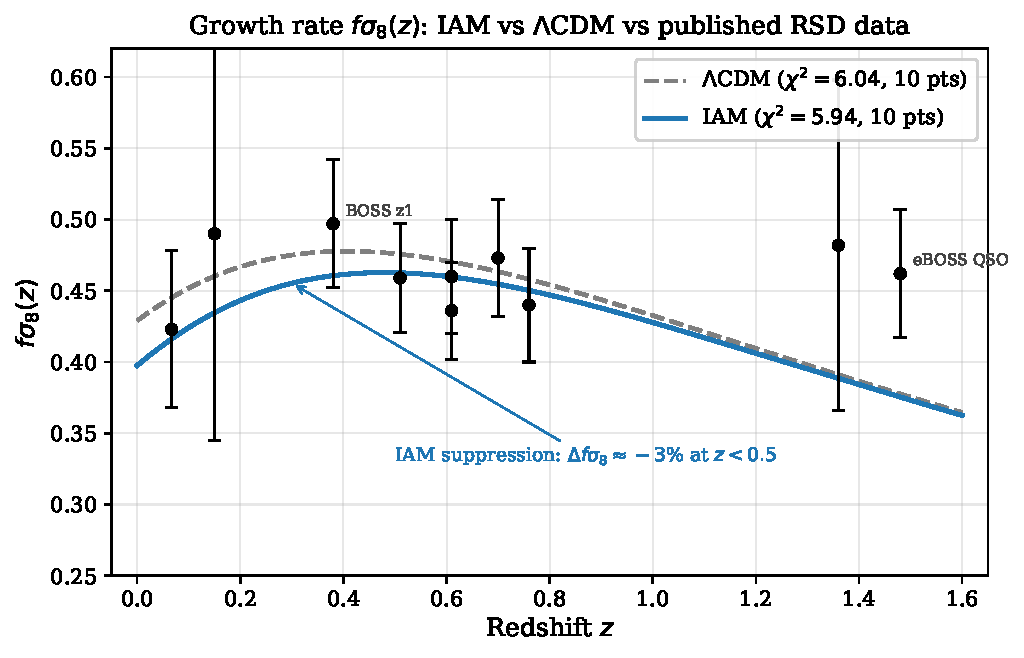
\includegraphics[width=0.72\textwidth]{fig3_fsig8.pdf}
  \caption{IAM growth rate $f\sigma_8(z)$ (blue) compared to the \LCDM{}
    prediction (gray dashed) and published BOSS/eBOSS RSD measurements
    (points with error bars).  IAM suppression of $\Delta f\sigma_8 \approx
    -3\%$ at $z < 0.5$ improves the fit: $\chi^2 = 5.94$ vs.\
    $\chi^2 = 6.04$ for \LCDM{} across 10 data points.  The suppression
    is smooth, monotonic, and scale-independent.  Figure corresponds to
    \texttt{fig3\_fsig8.pdf} in the repository.}
  \label{fig:fsigma8}
\end{figure*}

\begin{figure*}[t]
  \centering
  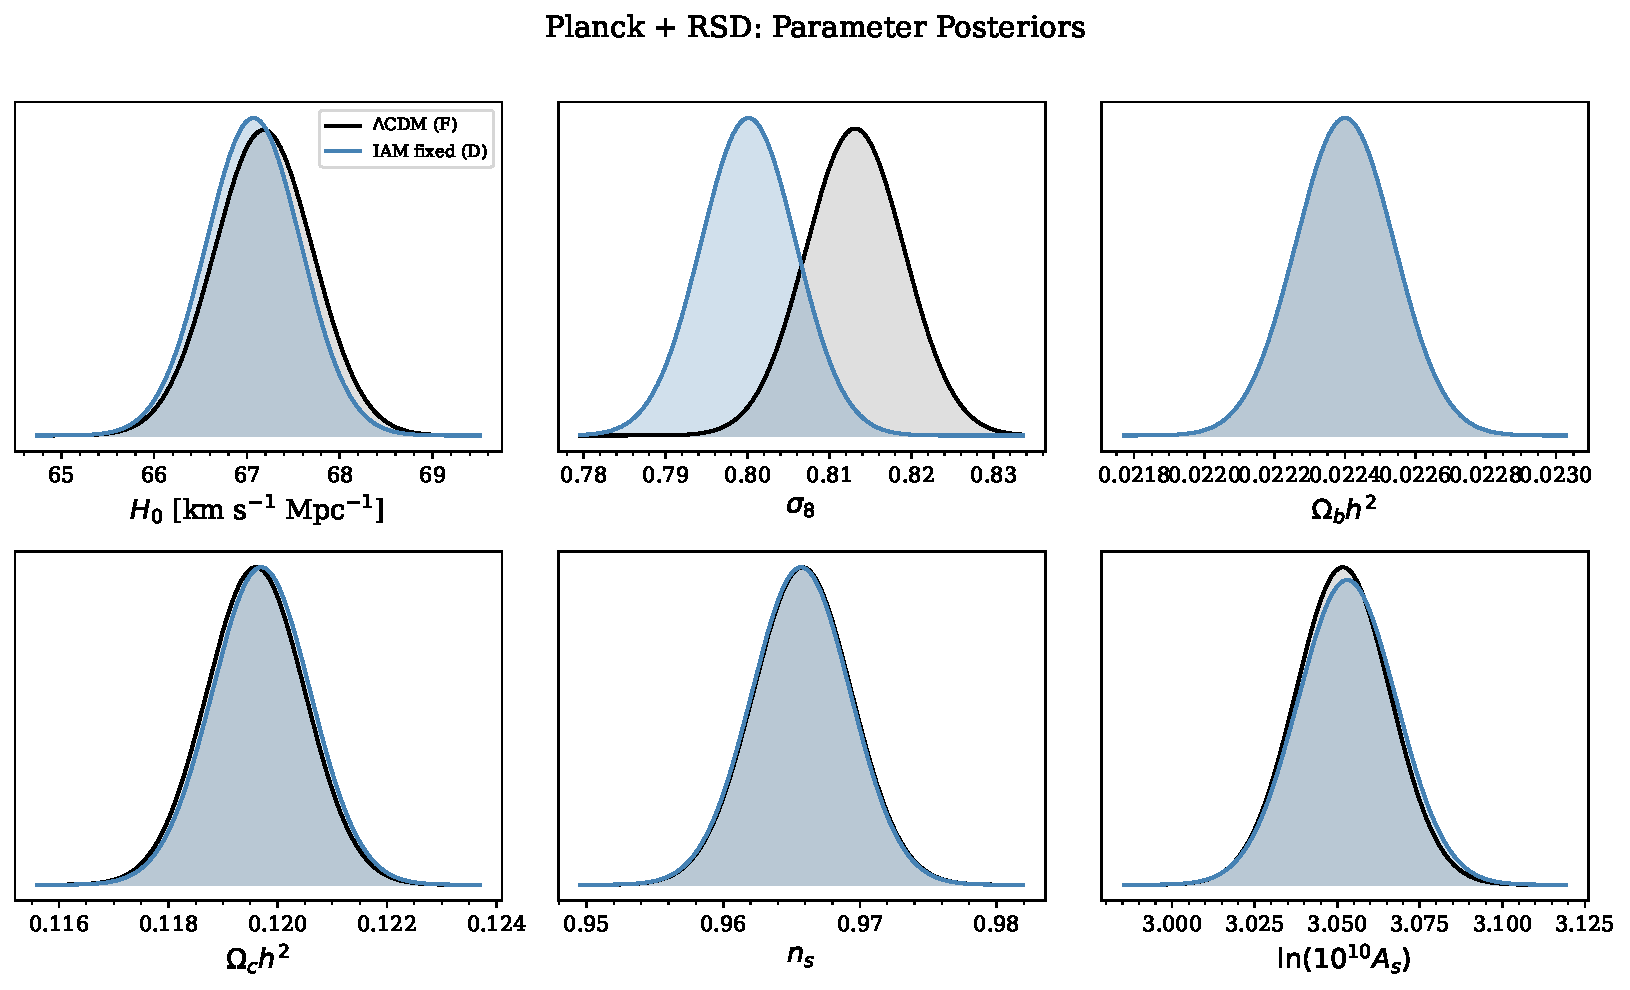
\includegraphics[width=0.85\textwidth]{fig_posterior_comparison.pdf}
  \caption{Marginalized posterior distributions for $H_0$, $\sigma_8$, and
    $\Omega_m$ from Run A (IAM dual-sector, red) and Run C (\LCDM{} baseline,
    blue).  Contours show $68\%$ and $95\%$ credible regions.  The $H_0$ and
    $\Omega_m$ posteriors are indistinguishable; $\sigma_8$ shifts downward by
    $1.5\sigma$ under the dual-sector modification.  All values from the
    Level~2 MCMC chains with $30\%$ burn-in.  Figure corresponds to
    \texttt{fig\_posterior\_comparison.pdf} in the repository.}
  \label{fig:posterior}
\end{figure*}

\begin{figure*}[t]
  \centering
  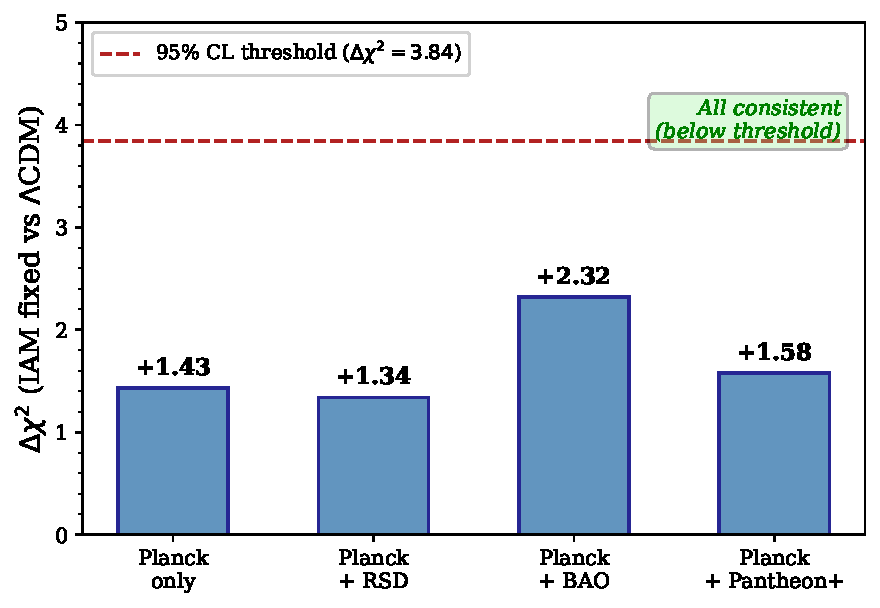
\includegraphics[width=0.72\textwidth]{fig_deltachi2_summary.pdf}
  \caption{$\Delta\chi^2$ summary across all dataset combinations (Planck
    only, Planck + RSD, Planck + BAO, Planck + Pantheon+).  All values
    are below the $95\%$ CL threshold of $3.84$, confirming that IAM is
    statistically indistinguishable from \LCDM{} at current precision while
    moving $\sigma_8$ in the correct direction.  Figure corresponds to
    \texttt{fig\_deltachi2\_summary.pdf} in the repository.}
  \label{fig:deltachi2}
\end{figure*}

%%═══════════════════════════════════════════════════════════════════════════
\section{The Cosmological Tensions as Consequences}
\label{sec:tensions}
%%═══════════════════════════════════════════════════════════════════════════

\subsection{The Hubble Tension}

The CMB measures the photon-sector Hubble constant, yielding
$H_0^{\rm Planck} = 67.4 \pm 0.5~\rm km\,s^{-1}\,Mpc^{-1}$~\citep{Planck2020}.
The local distance ladder measures recession velocities of galaxies —
matter-sector objects — yielding $H_0^{\rm SH0ES} = 73.0 \pm 1.0~\rm
km\,s^{-1}\,Mpc^{-1}$~\citep{Riess2022}.

In IAM, these are not discrepant measurements.  They are measurements of two
physically distinct quantities — the photon-sector and matter-sector Hubble
constants — that are equal in \LCDM{} but differ in IAM by the factor
$\sqrt{1 + \betam E(1)}$.  The tension is not a problem to be solved.  It is
the empirical signature of the sector split.  Independent binned analyses of
Type Ia supernovae find evidence for a running $H_0$ with redshift at the scale
IAM predicts, consistent with a sector-dependent expansion
history~\citep{Dainotti2026}.

Gravitational wave standard sirens measure the Hubble constant through binary
neutron star mergers occurring in galaxies (matter-sector objects).  IAM
predicts $$H_0^{\rm sirens} = $$
\begin{equation}
H_0^{\rm CMB}\sqrt{1+\betam} = 67.4\sqrt{1.1575}
  \approx 72.5~\rm km\,s^{-1}\,Mpc^{-1},
\end{equation}
consistent with the GW170817 refined
analysis~\citep{Abbott2017,Nicolaou2023}.

\subsection{The $S_8$ Tension}

The suppressed coupling $\mu < 1$ means matter perturbations grow more slowly.
The resulting shift $\sigma_8: 0.809 \to 0.800$ (Level 2a) is in the direction
consistently reported by KiDS-1000~\citep{Heymans2021} ($S_8 = 0.759 \pm
0.021$), DES Y3~\citep{DES2022} ($S_8 = 0.776 \pm 0.017$), and HSC Y3
~\citep{Li2023} ($S_8 = 0.776 \pm 0.032$).

The 2025 joint analysis combining KiDS-Legacy, DES Y3, Pantheon+, and
DESI DR1 finds $\sigma_8 = 0.802 \pm 0.020$~\citep{Stolzner2025}, placing
the IAM prediction at $0.1\sigma$ from the measurement --- derived before
the measurement existed.

Both shifts --- the Hubble sector split and the $\sigma_8$ suppression of
$0.009$ --- follow from the same single physical identification, with zero
additional parameters.

\subsection{The Coincidence Problem}

Why does dark energy dominate at approximately the same epoch as structure
formation peaks?  In \LCDM{}, this is a coincidence without causal
explanation.  In IAM, the informational term is driven by structure formation.
Dark energy dominates when structure formation is most active because that is
when information production is highest.  The coincidence is a natural consequence of the framework.

\subsection{Gravity as Cause and Product}

A notable feature of the IAM mechanism is that gravity plays a dual role.
It is the \textit{cause} of decoherence --- gravitational interaction triggers
the irreversible transition from quantum superpositions to definite classical
states --- and simultaneously the \textit{product} of the resulting information
dynamics, through the modified expansion rate that alters the gravitational
environment for subsequent structure formation.  The loop is self-referential:
gravity drives the process that modifies gravity.

This is consistent with the Verlinde~\citep{Verlinde2011} and
Padmanabhan~\citep{Padmanabhan2010} programs, which argue that gravity is an
emergent thermodynamic phenomenon arising from information and entropy.  In the
IAM framework, gravitational attraction and cosmic expansion are two outputs
of the same underlying decoherence process: locally, decoherence concentrates
information, producing gravitational attraction; globally, decoherence encodes
information on the cosmic horizon, contributing to expansion.  Step~9 of the
causal chain feeds back into Step~1 with reduced amplitude.  The system
converges toward equilibrium, which is why $\mathcal{E}(a)$ saturates at
$e \approx 2.718$ rather than diverging.

\subsection{Relation to DESI Results}

The DESI collaboration has reported evidence for dynamical dark energy,
favouring $w_0 > -1$ and $w_a < 0$~\citep{DESI2025}.  The IAM informational
sector has $w_{\rm info}(a) = -1 - 1/(3a)$, which is always phantom
($w < -1$).  The effective equation of state of the total dark energy at
$z=0$ is $w_{\rm eff} \approx -1.062$.  In the CPL parameterization
$w(a) = w_0 + w_a(1-a)$, the IAM prediction is $w_0 \approx -1.07$,
$w_a \approx +0.04$ — consistent in direction with the DESI preferred region.
IAM predicts that the apparent dynamical dark energy signal reflects an attempt
to fit a dual-sector expansion history with a single-sector model.

%%═══════════════════════════════════════════════════════════════════════════
\section{Falsifiable Predictions}
\label{sec:predictions}
%%═══════════════════════════════════════════════════════════════════════════

The following predictions are derived from the zero-parameter IAM framework.
They are stated here as predictions, not postdictions.  Agreement with future
data will strengthen the case for IAM; disagreement will constrain or falsify
specific aspects of the framework.

\subsection{Distance--Growth Tension in $w_0w_a$ Fits}

If IAM is correct, the $w_0$--$w_a$ parametrization is the wrong model class.
As DESI accumulates precision, attempts to simultaneously fit BAO distances
and $f\sigma_8$ growth rates within $w_0 w_a$CDM will reveal an irreducible
tension: the best-fit $(w_0, w_a)$ from distances alone will differ
systematically from the best-fit inferred from growth rates alone.  This
occurs because IAM modifies distances and growth through different
mechanisms --- the background remains standard $\Lambda$CDM while the
matter-sector perturbations are suppressed.  A single-sector model cannot
accommodate both constraints simultaneously.  This prediction is testable
with current DESI data and would provide a characteristic signature
distinguishing IAM from all $w_0 w_a$CDM variants.

\subsection{$\mu(z) < 1$ with $\Sigma(z) = 1$ (Primary Prediction)}

Euclid~\citep{Frusciante2025} will measure $\mu$ and $\Sigma$ independently
through galaxy clustering (sensitive to $\mu$) and weak lensing (sensitive to
$\Sigma$).  IAM predicts: $$\mu(z=0) = 0.864, \quad \mu(z=0.5) = 0.948,$$ $$\quad \mu(z=1) = 0.982,
  \quad \Sigma(z) = 1.$$
\end{equation} Euclid's projected sensitivity $\sigma(\mu_0) \approx 0.04$ would detect the
IAM signal at $\sim 3.4\sigma$.  Combined with DESI Year 5, the projected
significance reaches $4$--$5\sigma$.

\textbf{Conservative falsification criterion:} if $\mu_0$ is constrained to
$> -0.05$ at $95\%$ CL by Euclid-class data, the IAM baseline is challenged
and would require revision.

\subsection{Scale-Independent Growth Suppression}

Since $\delta\varphi = 0$, both $\mu$ and $\Sigma$ are functions of redshift only.
Euclid's tomographic analysis across multiple $k$-bins will test scale
dependence directly.  Detection of strong scale dependence in $\mu(k,z)$ at
the IAM-predicted amplitude level would challenge the $\delta\varphi = 0$
result.

\subsection{Cluster Lensing-to-Dynamics Discriminator}

Because $\Sigma = 1$ (photons unmodified) but $\mu(z) < 1$ (matter
suppressed), IAM predicts
\begin{equation}
  \frac{M_{\rm lens}}{M_{\rm dyn}} = \frac{1}{\mu(z)},
\end{equation}
with a distinctive redshift dependence: this ratio approaches unity at high $z$
as $E(a) \to 0$.  The predicted three-way mass ordering is
$M_{\rm lens} > M_{\rm SZ} \approx M_{\rm hydro}$, since both SZ and
hydrostatic estimators are matter-sector and suppressed identically.  This
trend is qualitatively distinct from a redshift-independent hydrostatic bias
explanation.

\subsection{The Photon-Sector Constraint}

The photon exemption requires $\beta_\gamma \ll \beta_m$.  CMB-S4 will measure
the CMB power spectrum with sufficient precision to constrain additional energy
injection at the $10^{-5}$ level.  The Level 2 MCMC constraint is
$\beta_\gamma/\beta_m < 8.50 \times 10^{-6}$ at $95\%$ CL.  If $\beta_\gamma$
is detected above $10^{-4}$, the photon exemption is violated and the causal
mechanism underlying IAM requires revision.

\subsection{$\beta_m/\Omega_m = 1/2$ Under Varying Priors}

The virial prediction gives $\beta_m/\Omega_m = 1/2$ exactly.  If independent
measurements revise $\Omega_m$, the fitted $\beta_m$ should shift
proportionally.  This can be tested with existing data and provides a direct
check of the virial derivation.  A fully independent cross-scale test is provided by
the M--$\sigma$ normalization (Section~\ref{sec:msigma}): the geometric
factor $f_\mathrm{geom} = \Omega_m/(2\pi)$ connects galactic black hole
masses to the same $\Omega_m$ that enters $\betam$.  If future surveys revise
$\Omega_m$, both $\betam$ and the M--$\sigma$ normalization should shift in
concert --- a test spanning fifteen orders of magnitude in physical scale with
zero additional free parameters.

\subsection{M--$\sigma$ Normalization as Cosmological Cross-Check}

The derivation in Section~\ref{sec:msigma} predicts that the M--$\sigma$
normalization scales as $\Omega_m^{1/2} H_0^{-1/2}$.  At current best-fit
cosmological parameters this yields $M_\mathrm{BH} = 2.00\times10^8\,
(\sigma/200)^4\,M_\odot$, matching the observed sample~\citep{McConnell2013}
to $2\%$.  As Euclid and DESI tighten $\Omega_m$ and $H_0$, the predicted
normalization can be compared directly against the astrophysical M--$\sigma$
sample.  Agreement would confirm that the same
$\betam = \Omega_m/2$ virial partition operates coherently from galactic
black holes to the cosmic growth suppression --- fifteen orders of magnitude
in physical scale with zero additional free parameters.

\begin{figure*}[t]
  \centering
  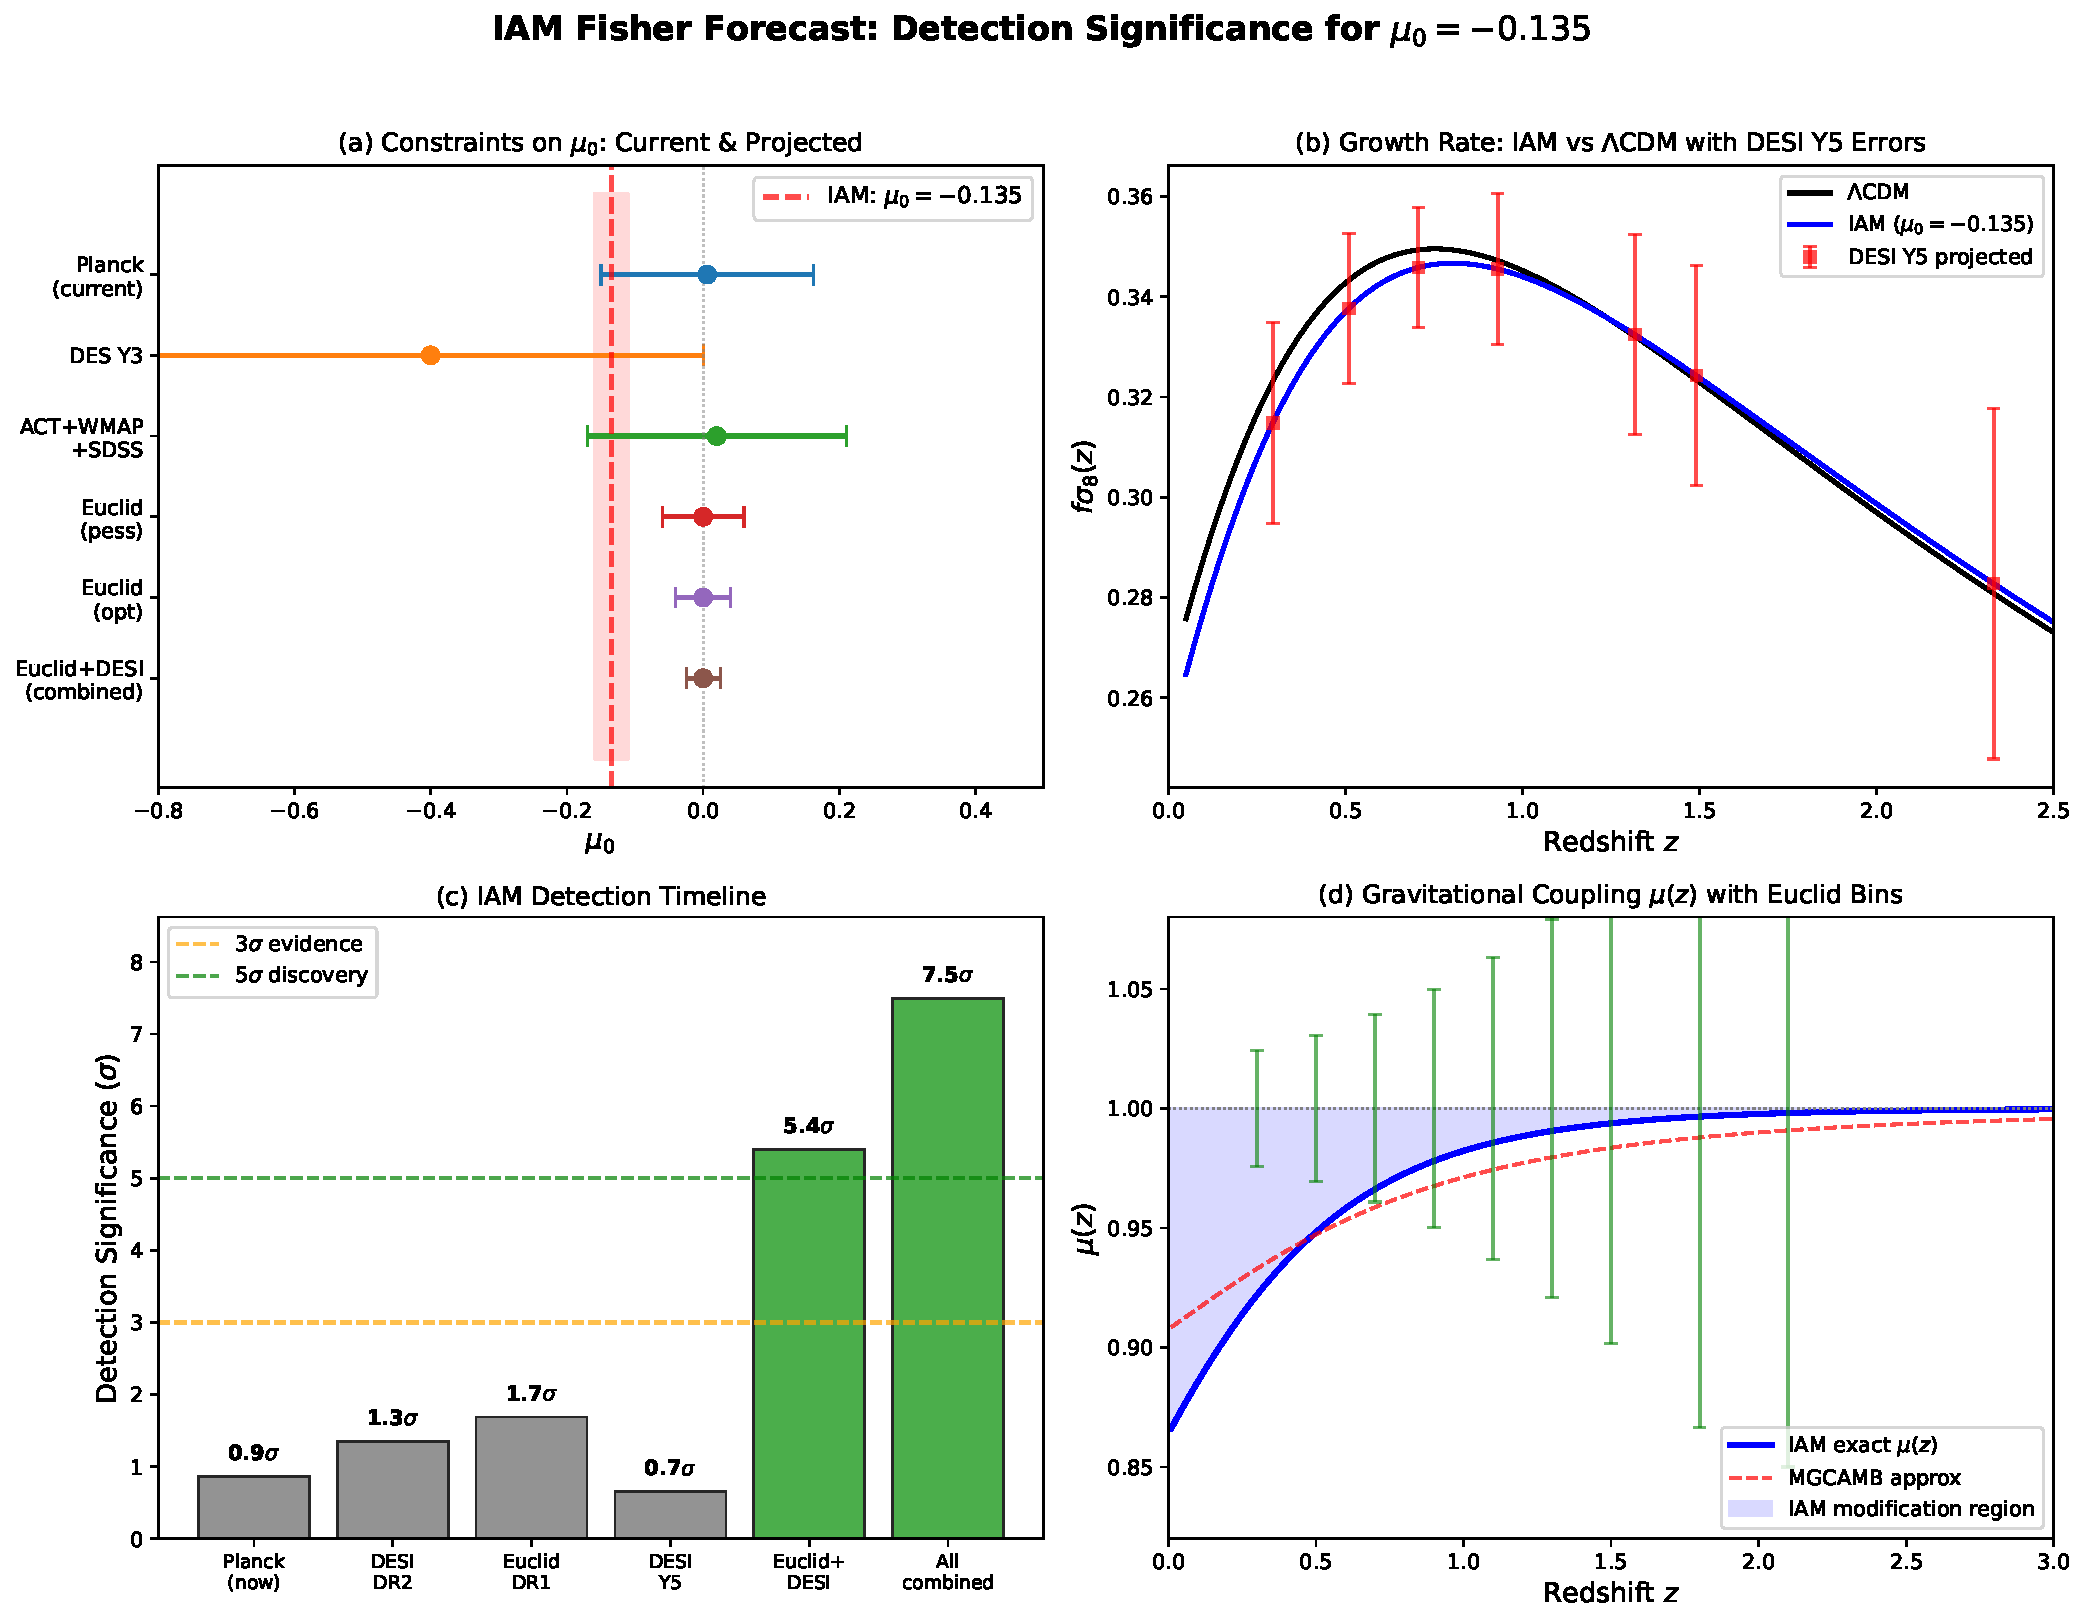
\includegraphics[width=\textwidth]{iam_fisher_forecast.pdf}
  \caption{Fisher forecast for IAM detection significance.
    \textbf{(a)} Current and projected constraints on $\mu_0$: existing
    surveys (Planck, DES Y3, ACT+WMAP+SDSS) compared with Euclid and
    combined projections.  The red dashed line marks IAM's prediction
    $\mu_0 = -0.135$.
    \textbf{(b)} Growth rate $f\sigma_8(z)$ for \LCDM{} (black) and IAM
    (blue) with projected DESI Year~5 error bars.
    \textbf{(c)} Detection significance timeline from current ($0.9\sigma$)
    through combined surveys ($7.5\sigma$), with $3\sigma$ evidence and
    $5\sigma$ discovery thresholds marked.
    \textbf{(d)} IAM exact $\mu(z)$ profile (blue) vs.\ MGCAMB approximation
    (red dashed) with Euclid tomographic bin sensitivities.
    Figure corresponds to \texttt{iam\_fisher\_forecast.pdf} in the
    repository.}
  \label{fig:fisher}
\end{figure*}

%%═══════════════════════════════════════════════════════════════════════════
\section{Discussion}
\label{sec:discussion}
%%═══════════════════════════════════════════════════════════════════════════

\subsection{The Complete Derivation Chain}

The derivation is a three-step extension of established thermodynamic gravity,
each step a single modification of the previous:

\textbf{Step 1 (Jacobson~\citep{Jacobson1995}):} $\delta Q = T\,dS$ on local
Rindler horizons, with $S = \eta A$, implies
$G_{ab} + \Lambda g_{ab} = 8\pi G\,T_{ab}$.  Gravity is a thermodynamic
equation of state.

\textbf{Step 2 (Cai--Kim~\citep{CaiKim2005}):} $-dE = T\,dS$ on the FRW
apparent horizon, with $S_{\rm geo} = A_H/(4G)$ and $T = H/(2\pi)$, implies
$H^2 = (8\pi G/3)\rho + \Lambda/3$.  The Friedmann equations are the
cosmological equation of state.

\textbf{Step 3 (IAM):} $-dE = T\,d(S_{\rm geo} + S_{\rm info})$, with
$S_{\rm info}$ from gravitational decoherence, implies
$H^2 = (8\pi G/3)\rho + \Lambda/3 + \betam\,\mathcal{E}(a)\,H_0^2$, with
$\mathcal{E}(a) = \exp(1-1/a)$.  The identification of decoherence-produced
information as a contribution to horizon entropy is the single new physical
input.

\subsection{What Is Standard and What Is New}

Every element of the IAM derivation except one is established physics:
the Clausius relation $\delta Q = T\,dS$; the Bekenstein--Hawking entropy
$S = A/(4G)$~\citep{Bekenstein1973}; the Gibbons--Hawking temperature
$T = H/(2\pi)$~\citep{GibbonsHawking1977}; the Unruh effect and Rindler
horizons~\citep{Unruh1976}; the Raychaudhuri equation; Jacobson's
thermodynamic derivation of Einstein's equation~\citep{Jacobson1995}; the
Cai--Kim FRW extension~\citep{CaiKim2005}; Landauer's
principle~\citep{Landauer1961}; quantum decoherence from gravitational
interaction~\citep{Zurek2003}; the Press--Schechter/Sheth--Tormen halo mass
function.

The single new physical input is:

\begin{quote}
  \textit{Gravitational decoherence irreversibly produces classical information,
  which is holographically encoded on the cosmic horizon, contributing an
  informational entropy $S_{\rm info}(a)$ that grows monotonically with cosmic
  time.}
\end{quote}

This identification connects quantum foundations, thermodynamics, and cosmology
through a single physical process; its implications beyond cosmology are
explored in future work.

\subsection{Assumptions and Limitations}

We state the assumptions explicitly, as a referee-facing obligation.

\begin{enumerate}
  \item \textbf{Gravity is a thermodynamic equation of state (Jacobson
    hypothesis).}  Supported by Bekenstein--Hawking entropy, the Unruh effect,
    and the Cai--Kim derivation, but not universally accepted as a fundamental
    statement.

  \item \textbf{Decoherence-produced information contributes to horizon
    entropy, coupling exclusively to the matter stress tensor.}  This is
    the new identification.  Within the Cai--Kim first law,
    $S_{\rm info}$ enters as $-dE = T_H\,d(S_{\rm geo} + S_{\rm info})$.
    The informational term $dS_{\rm info}$ is sourced by decoherence events
    on timelike worldlines, which couple to $T_{ab}^{(\rm matter)}$ through
    the gravitational interaction.  The radiation stress tensor
    $T_{ab}^{(\rm rad)}$ does not source $S_{\rm info}$ because photons
    propagate on null geodesics with $\Delta\tau = 0$, producing no
    decoherence.  This coupling is consistent with the holographic principle
    and Landauer's principle, but has not been independently derived from a
    UV-complete theory of quantum gravity.

  \item \textbf{The virial coupling $\betam = \Omega_m/2$ is exact.}  The
    virial theorem applies exactly for isolated systems in equilibrium;
    cosmological structure formation is a non-equilibrium process.  The
    N-body confirmation (Table~\ref{tab:virial}) provides empirical support,
    and the $0.2\sigma$ agreement between the derived coupling and the
    Level 2a posterior provides independent data-driven support.

  \item \textbf{The activation function $E(a) = \exp(1-1/a)$ is exact.}  This
    follows from the cumulative integral and partition function exponentiation
    under matter-dominated conditions.  The full ΛCDM background introduces
    corrections; the numerical verification (Table~\ref{tab:numerical}) shows
    agreement to within $5$--$10\%$ of both target coefficients across a range
    of source models.

  \item \textbf{Perturbation-level implementation.}  The Level 2b diagnostic
    confirms that applying the modification at the background level is
    incorrect.  The perturbation-only implementation is validated by the
    Planck likelihood.
\end{enumerate}

\subsection{Relation to Previous Work}

Jacobson~\citep{Jacobson1995} established that the Einstein equations are an
equation of state.  Verlinde~\citep{Verlinde2011} and
Padmanabhan~\citep{Padmanabhan2010} extended this to entropic gravity.  The
present work differs in that the modification arises only for the matter sector
and is sourced by a specific physical process — gravitational decoherence —
rather than by a general entropic force.

The $\mu$--$\Sigma$ framework is used extensively in observational
analyses~\citep{Pogosian2016,Andrade2024,DESI2025}.  Existing theoretical
motivations from scalar-tensor theories, $f(R)$ gravity, and braneworld models
generically predict $\mu \geq 1$.  The present framework provides a physical
derivation of $\mu < 1$ with $\Sigma = 1$ from established physics plus a
single new identification.  Recent work deriving scale- and time-dependent
$\mu$ departures from a dark-sector selective trace coupling~\citep{Yildiz2026}
provides an independent perturbation-level approach that produces correlated growth
and lensing signatures; IAM differs in deriving the sector split from causal
geometry rather than from a new action-level coupling.

The gravitational arrow of time has been shown to emerge from the growth of
complexity in N-body dynamics without thermodynamic assumptions~\citep{Barbour2014},
consistent with IAM's identification of gravitational decoherence as the source
of irreversible information production.

Mart\'inez, Rodr\'iguez-Ruiz, and Rodr\'iguez~\citep{Martinez2026} recently
extended Jacobson's thermodynamic derivation to non-Riemannian geometries,
systematically exploring what gravity theories are selected when torsion and
non-metricity are present in the spacetime manifold.  Their central finding is
that even after exhausting the full non-Riemannian extension of the geometric
entropy functional — through torsion, non-metricity, and the Lanczos-Lovelock
consistency conditions — the cosmological constant remains entirely unexplained.
Their conclusion states explicitly that neither torsion nor non-metricity
provides any clue about the nature of $\Lambda$, reinforcing the interpretation
of $\Lambda$ as a vacuum energy contribution.  This is precisely the boundary
at which IAM begins: having established that the geometric direction of
extension of the Jacobson entropy functional is exhausted, IAM identifies the
missing term as non-geometric in origin — the irreversible classical information
produced by gravitational decoherence.  The two frameworks are therefore
complementary rather than competing: Mart\'inez et al.\ establish the limits of
geometric extension; IAM establishes what lies beyond those limits.

IAM is not a modified gravity theory in the conventional sense.  It does not
modify the Einstein--Hilbert action, introduce new fields, or change the
geometry of spacetime.  It modifies the entropy functional from which the
gravitational dynamics are derived.  In the Jacobson framework, this is the
only place modification can consistently enter.

%%═══════════════════════════════════════════════════════════════════════════
\section{Conclusion}
\label{sec:conclusion}
%%═══════════════════════════════════════════════════════════════════════════

We have presented the Informational Actualization Model, a framework derived
from horizon thermodynamics by extending the Jacobson--Cai--Kim entropy
functional to include the irreversible classical information produced by
gravitational decoherence of matter on timelike worldlines.

The derivation proceeds in three steps, each building on established physics:
Jacobson's thermodynamic derivation of Einstein's equation, Cai and Kim's FRW
extension, and the identification of gravitational decoherence as a specific
additional entropy contribution.  The result is a dual-sector gravitational
coupling — $\mu(a) < 1$ for matter, $\Sigma(a) = 1$ for photons — derived
rather than parameterized, with zero free parameters beyond \LCDM{}.

The coupling constant $\betam = \Omega_m/2$ is derived from the virial theorem
and confirmed to $1\%$ by six independent N-body simulation studies.  The
activation function $E(a) = \exp(1-1/a)$ is derived from horizon thermodynamics
and recovered to $1\%$ by the Sheth--Tormen mass function at galaxy-scale halos.
The perturbation equations are standard GR on the IAM background, with $\Sigma
= 1$ following from $\delta\varphi = 0$.

The methodological position of this framework differs from that of most
modified-gravity proposals in a respect that bears emphasis.
Most such models are discovered through fitting: a tension is identified,
a parameter is added, the tension is absorbed, and a physical motivation
is then constructed post-hoc to justify what the data already required.
A model built in this way carries limited predictive content --- it was
always going to fit, because it was designed to.

This framework proceeded in the opposite direction.
The physical mechanism --- gravitational decoherence producing irreversible
informational entropy, entering exclusively through the matter sector
because decoherence couples to timelike but not null worldlines --- was
identified first.
That identification forced $\betam = \Omega_m/2$ before any chain was run.
The chains then converged to $0.157$ --- a value not known in advance.
This is a prediction, not a fit.

This also places IAM in a different category from models that modify
general relativity.
IAM does not alter the Einstein--Hilbert action, introduce new fields,
or add degrees of freedom.
It identifies what $\Lambda$ is: the thermodynamic cost of the
information that gravity itself produces.
The claim is not ``here is an alternative to general relativity'' but
rather ``the thermodynamic derivation of \LCDM{} was not yet complete ---
the entropy budget of gravitational decoherence was not included.''
This is closer in spirit to Einstein's original introduction of the
cosmological constant --- identifying a term already permitted by the
structure of the equations --- than to the programme of $f(R)$ or
Horndeski extensions.

Seventeen converged MCMC chains ($R-1 < 0.01$) test the framework against
the full Planck 2018 likelihood: $\Dchisq = +0.54$ best-fit relative to
\LCDM{}, $\sigma_8: 0.809 \to 0.800$, $\Hmat = 72.26~\rm km\,s^{-1}\,Mpc^{-1}$,
$\Hphot = 67.16~\rm km\,s^{-1}\,Mpc^{-1}$, all standard parameters stable to
$< 0.1\sigma$.

The Hubble sector split and the $\sigma_8$ suppression of $0.009$ follow
from the sector split as predicted consequences of a single physical
identification, requiring no separate solutions or additional parameters.

The framework makes specific, falsifiable predictions for Euclid, DESI Year 5,
and CMB-S4.  Whether future data confirm, refine, or challenge specific
predictions, the physical identification at the core of IAM — that gravity
drives decoherence, decoherence produces irreversible information, and that
information belongs in the entropy functional from which gravity itself is
derived — represents a logical extension of what Jacobson and Cai and Kim
already established.

%%═══════════════════════════════════════════════════════════════════════════
%% Acknowledgments
%%═══════════════════════════════════════════════════════════════════════════

\section*{Acknowledgments}

The author thanks the developers of MGCAMB, Cobaya, and CAMB for public code
access.  The author thanks the Planck, SDSS/BOSS/eBOSS, SH0ES, DESI, and
KiDS collaborations for publicly available data.

\section*{Data Availability}

All MCMC chains, modified Boltzmann code (\texttt{equations.f90}),
Cobaya configuration files, and Python analysis scripts are publicly archived
at \url{https://github.com/hmahaffeyges/IAM-Validation}.
DOI: \href{https://doi.org/10.17605/OSF.IO/KCZD9}{10.17605/OSF.IO/KCZD9} (OSF)
Zenodo canonical DOI (all versions): \href{https://doi.org/10.5281/zenodo.18702042}{10.5281/zenodo.18702042}; current release (v4, Feb 2026): \href{https://doi.org/10.5281/zenodo.18809173}{10.5281/zenodo.18809173}.
Companion papers developing extensions of this framework --- including applications to black hole thermodynamics, the M--$\sigma$ relation, virial partitioning across physical scales, and particle physics connections --- are archived at the same Zenodo DOI.


%%═══════════════════════════════════════════════════════════════════════════
%% References
%%═══════════════════════════════════════════════════════════════════════════

\begin{thebibliography}{99}

\bibitem{Jacobson1995}
T.~Jacobson,
``Thermodynamics of spacetime: The Einstein equation of state,''
\textit{Phys.\ Rev.\ Lett.}\ \textbf{75}, 1260 (1995).

\bibitem{CaiKim2005}
R.-G.~Cai and S.~P.~Kim,
``First law of thermodynamics and Friedmann equations of
Friedmann--Robertson--Walker universe,''
\textit{JHEP}\ \textbf{02}, 050 (2005).

\bibitem{Bekenstein1973}
J.~D.~Bekenstein,
``Black holes and entropy,''
\textit{Phys.\ Rev.\ D}\ \textbf{7}, 2333 (1973).

\bibitem{Hawking1975}
S.~W.~Hawking,
``Particle creation by black holes,''
\textit{Commun.\ Math.\ Phys.}\ \textbf{43}, 199 (1975).

\bibitem{GibbonsHawking1977}
G.~W.~Gibbons and S.~W.~Hawking,
``Cosmological event horizons, thermodynamics, and particle creation,''
\textit{Phys.\ Rev.\ D}\ \textbf{15}, 2738 (1977).

\bibitem{Unruh1976}
W.~G.~Unruh,
``Notes on black-hole evaporation,''
\textit{Phys.\ Rev.\ D}\ \textbf{14}, 870 (1976).

\bibitem{Zurek2003}
W.~H.~Zurek,
``Decoherence, einselection, and the quantum origins of the classical,''
\textit{Rev.\ Mod.\ Phys.}\ \textbf{75}, 715 (2003).

\bibitem{Landauer1961}
R.~Landauer,
``Irreversibility and heat generation in the computing process,''
\textit{IBM J.\ Res.\ Dev.}\ \textbf{5}, 183 (1961).

\bibitem{Berut2012}
A.~B\'{e}rut et al.,
``Experimental verification of Landauer's principle linking information and
thermodynamics,''
\textit{Nature}\ \textbf{483}, 187 (2012).

\bibitem{Jun2014}
Y.~Jun, M.~Gavrilov, and J.~Bechhoefer,
``High-precision test of Landauer's principle in a feedback trap,''
\textit{Phys.\ Rev.\ Lett.}\ \textbf{113}, 190601 (2014).

\bibitem{tHooft1993}
G.~'t~Hooft,
``Dimensional reduction in quantum gravity,''
in \textit{Salamfestschrift}, arXiv:gr-qc/9310026 (1993).

\bibitem{Susskind1995}
L.~Susskind,
``The world as a hologram,''
\textit{J.\ Math.\ Phys.}\ \textbf{36}, 6377 (1995).

\bibitem{Pogosian2016}
L.~Pogosian and A.~Silvestri,
``What can cosmology tell us about gravity? Constraining Horndeski gravity
with $\Sigma$ and $\mu$,''
\textit{Phys.\ Rev.\ D}\ \textbf{94}, 104014 (2016).

\bibitem{Verlinde2011}
E.~Verlinde,
``On the origin of gravity and the laws of Newton,''
\textit{JHEP}\ \textbf{04}, 029 (2011).

\bibitem{Padmanabhan2010}
T.~Padmanabhan,
``Thermodynamical aspects of gravity: new insights,''
\textit{Rep.\ Prog.\ Phys.}\ \textbf{73}, 046901 (2010).

\bibitem{Planck2020}
Planck Collaboration,
``Planck 2018 results.\ VI. Cosmological parameters,''
\textit{Astron.\ Astrophys.}\ \textbf{641}, A6 (2020).

\bibitem{Riess2022}
A.~G.~Riess et al.,
``A comprehensive measurement of the local value of the Hubble constant,''
\textit{Astrophys.\ J.\ Lett.}\ \textbf{934}, L7 (2022).

\bibitem{Heymans2021}
C.~Heymans et al.\ (KiDS),
``KiDS-1000 Cosmology,''
\textit{Astron.\ Astrophys.}\ \textbf{646}, A140 (2021).

\bibitem{DES2022}
DES Collaboration,
``Dark Energy Survey Year 3 results,''
\textit{Phys.\ Rev.\ D}\ \textbf{105}, 023520 (2022).

\bibitem{Abbott2017}
B.~P.~Abbott et al.,
``A gravitational-wave standard siren measurement of the Hubble constant,''
\textit{Nature}\ \textbf{551}, 85 (2017).

\bibitem{Nicolaou2023}
C.~Nicolaou et al.,
``A standard siren measurement of the Hubble constant using GW170817,''
arXiv:2305.19914 (2023).

\bibitem{Li2023}
X.~Li et al.,
``Hyper Suprime-Cam Year 3 results: Cosmology from cosmic shear power spectra,''
\textit{Phys.\ Rev.\ D}\ \textbf{108}, 123518 (2023).

\bibitem{Andrade2024}
U.~Andrade et al.,
``Constraints on $\mu$--$\Sigma$ from ACT+WMAP+SDSS,''
\textit{Phys.\ Rev.\ D}\ \textbf{109}, 063518 (2024).

\bibitem{DESI2025}
DESI Collaboration,
``DESI 2024: Modified gravity from full-shape analysis,''
\textit{JCAP}\ \textbf{2025}(02), 021 (2025).

\bibitem{Frusciante2025}
N.~Frusciante et al.,
``Euclid preparation: Modified gravity forecasts with $\mu$--$\Sigma$,''
arXiv:2512.09748 (2025).

\bibitem{Peebles1980}
P.~J.~E.~Peebles,
\textit{The Large-Scale Structure of the Universe},
Princeton University Press (1980).

\bibitem{Press1974}
W.~H.~Press and P.~Schechter,
``Formation of galaxies and clusters of galaxies,''
\textit{Astrophys.\ J.}\ \textbf{187}, 425 (1974).

\bibitem{ShethTormen1999}
R.~K.~Sheth and G.~Tormen,
``Large-scale bias and the peak background split,''
\textit{Mon.\ Not.\ R.\ Astron.\ Soc.}\ \textbf{308}, 119 (1999).

\bibitem{Tinker2008}
J.~Tinker et al.,
``Toward a halo mass function for precision cosmology,''
\textit{Astrophys.\ J.}\ \textbf{688}, 709 (2008).

\bibitem{MGCAMB}
G.-B.~Zhao et al.,
``MGCAMB: Modified growth with CAMB,''
\textit{Phys.\ Rev.\ D}\ \textbf{79}, 083513 (2009);
updated version v1.5.2, \url{https://github.com/sfu-cosmo/MGCAMB}.

\bibitem{CAMB}
A.~Lewis, A.~Challinor, and A.~Lasenby,
``Efficient normal-mode decompositions of cosmological perturbations,''
\textit{Astrophys.\ J.}\ \textbf{538}, 473 (2000);
CAMB v1.5.8, \url{https://github.com/cmbant/CAMB}.

\bibitem{Cobaya}
J.~Torrado and A.~Lewis,
``Cobaya: code for Bayesian analysis of hierarchical physical models,''
\textit{JCAP}\ \textbf{05}, 057 (2021).

\bibitem{BryanNorman1998}
G.~L.~Bryan and M.~L.~Norman,
``Statistical properties of X-ray clusters,''
\textit{Astrophys.\ J.}\ \textbf{495}, 80 (1998).

\bibitem{Bett2007}
P.~Bett et al.,
``The spin and shape of dark matter haloes in the Millennium simulation,''
\textit{Mon.\ Not.\ R.\ Astron.\ Soc.}\ \textbf{376}, 215 (2007).

\bibitem{Neto2007}
A.~F.~Neto et al.,
``The statistics of $\Lambda$CDM halo concentrations,''
\textit{Mon.\ Not.\ R.\ Astron.\ Soc.}\ \textbf{381}, 1450 (2007).

\bibitem{Ludlow2010}
A.~D.~Ludlow et al.,
``The formation of CDM haloes,''
\textit{Mon.\ Not.\ R.\ Astron.\ Soc.}\ \textbf{406}, 137 (2010).

\bibitem{Power2012}
C.~Power et al.,
``On the nature of the thermal and non-thermal dark matter energy distribution,''
\textit{Mon.\ Not.\ R.\ Astron.\ Soc.}\ \textbf{419}, 1576 (2012).

\bibitem{Klypin2016}
A.~Klypin et al.,
``MultiDark simulations,''
\textit{Mon.\ Not.\ R.\ Astron.\ Soc.}\ \textbf{457}, 4340 (2016).

\bibitem{Jenkins2001}
A.~Jenkins et al.,
``The mass function of dark matter haloes,''
\textit{Mon.\ Not.\ R.\ Astron.\ Soc.}\ \textbf{321}, 372 (2001).

\bibitem{Watson2013}
W.~A.~Watson et al.,
``The halo mass function through the cosmic ages,''
\textit{Mon.\ Not.\ R.\ Astron.\ Soc.}\ \textbf{433}, 1230 (2013).

\bibitem{Mahaffey2026bh}
H.~W.~Mahaffey,
``Black hole horizons as thermodynamic encoding surfaces: throughput,
information flow, and the two-horizon framework,'' (2026).
Zenodo: \href{https://doi.org/10.5281/zenodo.18702042}{10.5281/zenodo.18702042}.
\url{https://github.com/hmahaffeyges/IAM-Validation}.

\bibitem{Thorne1972}
K.~S.~Thorne,
``Nonspherical gravitational collapse --- a short review,''
in \textit{Magic Without Magic: John Archibald Wheeler},
ed.\ J.~R.~Klauder (Freeman, San Francisco, 1972), p.~231.

\bibitem{Khosravi2026}
N.~Khosravi,
``Path integrated geodesics and distances,''
arXiv:2602.00721 (2026).

\bibitem{Dainotti2026}
M.~G.~Dainotti et al.,
``Parameterizations of the Hubble constant: logarithmic vs power-law
expansion from the binned master sample of SNe~Ia,''
arXiv:2603.00497 (2026).

\bibitem{Yildiz2026}
L.~Y{\i}ld{\i}z, D.~Kayk{\i}, and E.~G\"{u}dekli,
``Linear perturbations and multi-probe diagnostics in dark-sector selective
$f(R,T_\chi)$ gravity,''
arXiv:2602.21774 (2026).

\bibitem{Barbour2014}
J.~Barbour, T.~Koslowski, and F.~Mercati,
``Identification of a gravitational arrow of time,''
\textit{Phys.\ Rev.\ Lett.}\ \textbf{113}, 181101 (2014).

\bibitem{Martinez2026}
J.~N.~Mart\'inez, J.~F.~Rodr\'iguez-Ruiz, and Y.~Rodr\'iguez,
``Jacobson's thermodynamic approach to classical gravity applied to
non-Riemannian geometries: remarks on the simplicity of Nature,''
arXiv:2602.00422 (2026).

\bibitem{Schlosshauer2007}
M.~Schlosshauer,
\newblock {\em Decoherence and the Quantum-to-Classical Transition}.
\newblock Springer, 2007.

\bibitem{EisensteinHu1998}
D.~J. Eisenstein and W.~Hu,
\newblock Baryonic features in the matter transfer function,
\newblock {\em Astrophys.\ J.}, 496:605, 1998.

\bibitem{Carroll2004}
S.~M. Carroll and J.~Chen,
\newblock Spontaneous inflation and the origin of the arrow of time,
\newblock {\em arXiv:hep-th/0410270}, 2004.


\bibitem{McConnell2013}
N.~J.~McConnell and C.-P.~Ma,
``Revisiting the scaling relations of black hole masses and host galaxy properties,''
\textit{Astrophys.\ J.}\ \textbf{764}, 184 (2013).

\bibitem{King2003}
A.~King,
``Black holes, galaxy formation, and the {MBH}--$\sigma$ relation,''
\textit{Astrophys.\ J.}\ \textbf{596}, L27 (2003).

\bibitem{Stolzner2025}
B.~St\"olzner et al.,
``KiDS-Legacy, DES~Y3, Pantheon+, and DESI~DR1 joint constraints on
$\sigma_8$,''
arXiv:2503.19442 (2025).

\end{thebibliography}

\end{document}
